% Created by tikzDevice version 0.12.6 on 2025-02-12 17:48:24
% !TEX encoding = UTF-8 Unicode
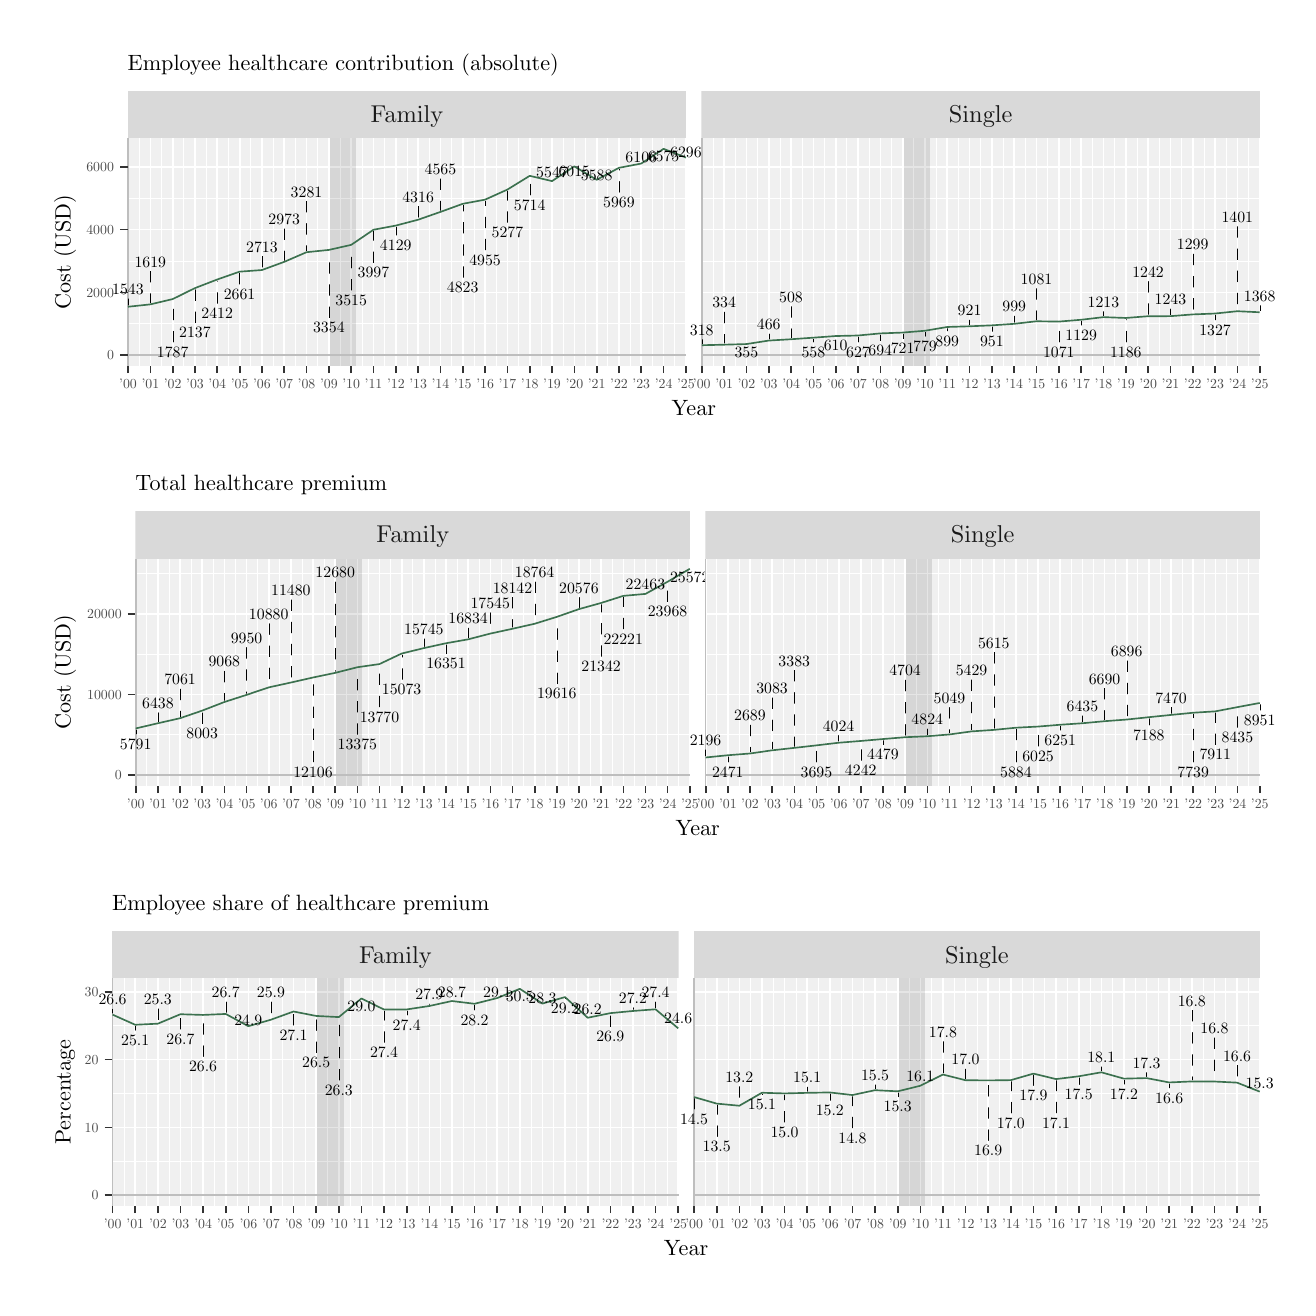
\begin{tikzpicture}[x=1pt,y=1pt]
\definecolor{fillColor}{RGB}{255,255,255}
\path[use as bounding box,fill=fillColor,fill opacity=0.00] (0,0) rectangle (455.30,455.30);
\begin{scope}
\path[clip] (  0.00,303.53) rectangle (455.30,455.30);
\definecolor{drawColor}{RGB}{255,255,255}
\definecolor{fillColor}{RGB}{255,255,255}

\path[draw=drawColor,line width= 0.6pt,line join=round,line cap=round,fill=fillColor] (  0.00,303.53) rectangle (455.30,455.30);
\end{scope}
\begin{scope}
\path[clip] (  0.00,  0.00) rectangle (455.30,455.30);
\definecolor{fillColor}{gray}{0.94}

\path[fill=fillColor] ( 36.14,333.22) rectangle (237.97,415.25);
\definecolor{drawColor}{RGB}{255,255,255}

\path[draw=drawColor,line width= 0.3pt,line join=round] ( 36.14,348.29) --
	(237.97,348.29);

\path[draw=drawColor,line width= 0.3pt,line join=round] ( 36.14,370.97) --
	(237.97,370.97);

\path[draw=drawColor,line width= 0.3pt,line join=round] ( 36.14,393.66) --
	(237.97,393.66);

\path[draw=drawColor,line width= 0.3pt,line join=round] ( 40.31,333.22) --
	( 40.31,415.25);

\path[draw=drawColor,line width= 0.3pt,line join=round] ( 48.38,333.22) --
	( 48.38,415.25);

\path[draw=drawColor,line width= 0.3pt,line join=round] ( 56.44,333.22) --
	( 56.44,415.25);

\path[draw=drawColor,line width= 0.3pt,line join=round] ( 64.50,333.22) --
	( 64.50,415.25);

\path[draw=drawColor,line width= 0.3pt,line join=round] ( 72.57,333.22) --
	( 72.57,415.25);

\path[draw=drawColor,line width= 0.3pt,line join=round] ( 80.64,333.22) --
	( 80.64,415.25);

\path[draw=drawColor,line width= 0.3pt,line join=round] ( 88.69,333.22) --
	( 88.69,415.25);

\path[draw=drawColor,line width= 0.3pt,line join=round] ( 96.75,333.22) --
	( 96.75,415.25);

\path[draw=drawColor,line width= 0.3pt,line join=round] (104.82,333.22) --
	(104.82,415.25);

\path[draw=drawColor,line width= 0.3pt,line join=round] (112.89,333.22) --
	(112.89,415.25);

\path[draw=drawColor,line width= 0.3pt,line join=round] (120.95,333.22) --
	(120.95,415.25);

\path[draw=drawColor,line width= 0.3pt,line join=round] (129.01,333.22) --
	(129.01,415.25);

\path[draw=drawColor,line width= 0.3pt,line join=round] (137.08,333.22) --
	(137.08,415.25);

\path[draw=drawColor,line width= 0.3pt,line join=round] (145.15,333.22) --
	(145.15,415.25);

\path[draw=drawColor,line width= 0.3pt,line join=round] (153.20,333.22) --
	(153.20,415.25);

\path[draw=drawColor,line width= 0.3pt,line join=round] (161.26,333.22) --
	(161.26,415.25);

\path[draw=drawColor,line width= 0.3pt,line join=round] (169.33,333.22) --
	(169.33,415.25);

\path[draw=drawColor,line width= 0.3pt,line join=round] (177.40,333.22) --
	(177.40,415.25);

\path[draw=drawColor,line width= 0.3pt,line join=round] (185.46,333.22) --
	(185.46,415.25);

\path[draw=drawColor,line width= 0.3pt,line join=round] (193.52,333.22) --
	(193.52,415.25);

\path[draw=drawColor,line width= 0.3pt,line join=round] (201.59,333.22) --
	(201.59,415.25);

\path[draw=drawColor,line width= 0.3pt,line join=round] (209.66,333.22) --
	(209.66,415.25);

\path[draw=drawColor,line width= 0.3pt,line join=round] (217.71,333.22) --
	(217.71,415.25);

\path[draw=drawColor,line width= 0.3pt,line join=round] (225.77,333.22) --
	(225.77,415.25);

\path[draw=drawColor,line width= 0.3pt,line join=round] (233.84,333.22) --
	(233.84,415.25);

\path[draw=drawColor,line width= 0.6pt,line join=round] ( 36.14,336.95) --
	(237.97,336.95);

\path[draw=drawColor,line width= 0.6pt,line join=round] ( 36.14,359.63) --
	(237.97,359.63);

\path[draw=drawColor,line width= 0.6pt,line join=round] ( 36.14,382.32) --
	(237.97,382.32);

\path[draw=drawColor,line width= 0.6pt,line join=round] ( 36.14,405.00) --
	(237.97,405.00);

\path[draw=drawColor,line width= 0.6pt,line join=round] ( 36.27,333.22) --
	( 36.27,415.25);

\path[draw=drawColor,line width= 0.6pt,line join=round] ( 44.35,333.22) --
	( 44.35,415.25);

\path[draw=drawColor,line width= 0.6pt,line join=round] ( 52.41,333.22) --
	( 52.41,415.25);

\path[draw=drawColor,line width= 0.6pt,line join=round] ( 60.47,333.22) --
	( 60.47,415.25);

\path[draw=drawColor,line width= 0.6pt,line join=round] ( 68.53,333.22) --
	( 68.53,415.25);

\path[draw=drawColor,line width= 0.6pt,line join=round] ( 76.61,333.22) --
	( 76.61,415.25);

\path[draw=drawColor,line width= 0.6pt,line join=round] ( 84.66,333.22) --
	( 84.66,415.25);

\path[draw=drawColor,line width= 0.6pt,line join=round] ( 92.72,333.22) --
	( 92.72,415.25);

\path[draw=drawColor,line width= 0.6pt,line join=round] (100.78,333.22) --
	(100.78,415.25);

\path[draw=drawColor,line width= 0.6pt,line join=round] (108.86,333.22) --
	(108.86,415.25);

\path[draw=drawColor,line width= 0.6pt,line join=round] (116.92,333.22) --
	(116.92,415.25);

\path[draw=drawColor,line width= 0.6pt,line join=round] (124.98,333.22) --
	(124.98,415.25);

\path[draw=drawColor,line width= 0.6pt,line join=round] (133.04,333.22) --
	(133.04,415.25);

\path[draw=drawColor,line width= 0.6pt,line join=round] (141.12,333.22) --
	(141.12,415.25);

\path[draw=drawColor,line width= 0.6pt,line join=round] (149.17,333.22) --
	(149.17,415.25);

\path[draw=drawColor,line width= 0.6pt,line join=round] (157.23,333.22) --
	(157.23,415.25);

\path[draw=drawColor,line width= 0.6pt,line join=round] (165.29,333.22) --
	(165.29,415.25);

\path[draw=drawColor,line width= 0.6pt,line join=round] (173.37,333.22) --
	(173.37,415.25);

\path[draw=drawColor,line width= 0.6pt,line join=round] (181.43,333.22) --
	(181.43,415.25);

\path[draw=drawColor,line width= 0.6pt,line join=round] (189.49,333.22) --
	(189.49,415.25);

\path[draw=drawColor,line width= 0.6pt,line join=round] (197.55,333.22) --
	(197.55,415.25);

\path[draw=drawColor,line width= 0.6pt,line join=round] (205.63,333.22) --
	(205.63,415.25);

\path[draw=drawColor,line width= 0.6pt,line join=round] (213.68,333.22) --
	(213.68,415.25);

\path[draw=drawColor,line width= 0.6pt,line join=round] (221.74,333.22) --
	(221.74,415.25);

\path[draw=drawColor,line width= 0.6pt,line join=round] (229.80,333.22) --
	(229.80,415.25);

\path[draw=drawColor,line width= 0.6pt,line join=round] (237.88,333.22) --
	(237.88,415.25);
\definecolor{fillColor}{RGB}{190,190,190}

\path[fill=fillColor,fill opacity=0.01] (109.28,333.22) rectangle (118.71,415.25);

\path[fill=fillColor,fill opacity=0.01] (109.28,333.22) rectangle (118.71,415.25);

\path[fill=fillColor,fill opacity=0.01] (109.28,333.22) rectangle (118.71,415.25);

\path[fill=fillColor,fill opacity=0.01] (109.28,333.22) rectangle (118.71,415.25);

\path[fill=fillColor,fill opacity=0.01] (109.28,333.22) rectangle (118.71,415.25);

\path[fill=fillColor,fill opacity=0.01] (109.28,333.22) rectangle (118.71,415.25);

\path[fill=fillColor,fill opacity=0.01] (109.28,333.22) rectangle (118.71,415.25);

\path[fill=fillColor,fill opacity=0.01] (109.28,333.22) rectangle (118.71,415.25);

\path[fill=fillColor,fill opacity=0.01] (109.28,333.22) rectangle (118.71,415.25);

\path[fill=fillColor,fill opacity=0.01] (109.28,333.22) rectangle (118.71,415.25);

\path[fill=fillColor,fill opacity=0.01] (109.28,333.22) rectangle (118.71,415.25);

\path[fill=fillColor,fill opacity=0.01] (109.28,333.22) rectangle (118.71,415.25);

\path[fill=fillColor,fill opacity=0.01] (109.28,333.22) rectangle (118.71,415.25);

\path[fill=fillColor,fill opacity=0.01] (109.28,333.22) rectangle (118.71,415.25);

\path[fill=fillColor,fill opacity=0.01] (109.28,333.22) rectangle (118.71,415.25);

\path[fill=fillColor,fill opacity=0.01] (109.28,333.22) rectangle (118.71,415.25);

\path[fill=fillColor,fill opacity=0.01] (109.28,333.22) rectangle (118.71,415.25);

\path[fill=fillColor,fill opacity=0.01] (109.28,333.22) rectangle (118.71,415.25);

\path[fill=fillColor,fill opacity=0.01] (109.28,333.22) rectangle (118.71,415.25);

\path[fill=fillColor,fill opacity=0.01] (109.28,333.22) rectangle (118.71,415.25);

\path[fill=fillColor,fill opacity=0.01] (109.28,333.22) rectangle (118.71,415.25);

\path[fill=fillColor,fill opacity=0.01] (109.28,333.22) rectangle (118.71,415.25);

\path[fill=fillColor,fill opacity=0.01] (109.28,333.22) rectangle (118.71,415.25);

\path[fill=fillColor,fill opacity=0.01] (109.28,333.22) rectangle (118.71,415.25);

\path[fill=fillColor,fill opacity=0.01] (109.28,333.22) rectangle (118.71,415.25);

\path[fill=fillColor,fill opacity=0.01] (109.28,333.22) rectangle (118.71,415.25);
\definecolor{drawColor}{RGB}{190,190,190}

\path[draw=drawColor,line width= 0.6pt,line join=round] ( 36.14,336.95) -- (237.97,336.95);

\path[draw=drawColor,line width= 0.6pt,line join=round] ( 36.25,333.22) -- ( 36.25,415.25);
\definecolor{drawColor}{RGB}{60,113,79}

\path[draw=drawColor,line width= 0.6pt,line join=round] ( 36.25,354.45) --
	( 44.33,355.31) --
	( 52.39,357.22) --
	( 60.45,361.19) --
	( 68.50,364.30) --
	( 76.58,367.13) --
	( 84.64,367.72) --
	( 92.70,370.67) --
	(100.76,374.16) --
	(108.84,374.99) --
	(116.90,376.81) --
	(124.96,382.28) --
	(133.01,383.78) --
	(141.09,385.90) --
	(149.15,388.72) --
	(157.21,391.65) --
	(165.27,393.15) --
	(173.35,396.80) --
	(181.41,401.76) --
	(189.47,399.86) --
	(197.52,405.17) --
	(205.60,400.33) --
	(213.66,404.65) --
	(221.72,406.20) --
	(229.78,411.52) --
	(237.86,408.36);
\definecolor{drawColor}{RGB}{0,0,0}

\path[draw=drawColor,line width= 0.1pt,dash pattern=on 4pt off 4pt ,line join=round,line cap=round] ( 36.25,357.33) -- ( 36.25,354.97);

\path[draw=drawColor,line width= 0.1pt,dash pattern=on 4pt off 4pt ,line join=round,line cap=round] ( 44.33,367.27) -- ( 44.33,355.83);

\path[draw=drawColor,line width= 0.1pt,dash pattern=on 4pt off 4pt ,line join=round,line cap=round] ( 52.39,341.65) -- ( 52.39,356.70);

\path[draw=drawColor,line width= 0.1pt,dash pattern=on 4pt off 4pt ,line join=round,line cap=round] ( 60.45,348.64) -- ( 60.45,360.67);

\path[draw=drawColor,line width= 0.1pt,dash pattern=on 4pt off 4pt ,line join=round,line cap=round] ( 68.50,355.62) -- ( 68.50,363.79);

\path[draw=drawColor,line width= 0.1pt,dash pattern=on 4pt off 4pt ,line join=round,line cap=round] ( 76.58,362.60) -- ( 76.58,366.61);

\path[draw=drawColor,line width= 0.1pt,dash pattern=on 4pt off 4pt ,line join=round,line cap=round] ( 84.64,372.70) -- ( 84.64,368.24);

\path[draw=drawColor,line width= 0.1pt,dash pattern=on 4pt off 4pt ,line join=round,line cap=round] ( 92.70,382.64) -- ( 92.70,371.18);

\path[draw=drawColor,line width= 0.1pt,dash pattern=on 4pt off 4pt ,line join=round,line cap=round] (100.76,392.58) -- (100.76,374.68);

\path[draw=drawColor,line width= 0.1pt,dash pattern=on 4pt off 4pt ,line join=round,line cap=round] (108.84,350.48) -- (108.84,374.47);

\path[draw=drawColor,line width= 0.1pt,dash pattern=on 4pt off 4pt ,line join=round,line cap=round] (116.90,360.41) -- (116.90,376.30);

\path[draw=drawColor,line width= 0.1pt,dash pattern=on 4pt off 4pt ,line join=round,line cap=round] (124.96,370.35) -- (124.96,381.76);

\path[draw=drawColor,line width= 0.1pt,dash pattern=on 4pt off 4pt ,line join=round,line cap=round] (133.01,380.26) -- (133.01,383.26);

\path[draw=drawColor,line width= 0.1pt,dash pattern=on 4pt off 4pt ,line join=round,line cap=round] (141.09,390.75) -- (141.09,386.42);

\path[draw=drawColor,line width= 0.1pt,dash pattern=on 4pt off 4pt ,line join=round,line cap=round] (149.15,400.69) -- (149.15,389.24);

\path[draw=drawColor,line width= 0.1pt,dash pattern=on 4pt off 4pt ,line join=round,line cap=round] (157.21,364.98) -- (157.21,391.13);

\path[draw=drawColor,line width= 0.1pt,dash pattern=on 4pt off 4pt ,line join=round,line cap=round] (165.27,374.92) -- (165.27,392.63);

\path[draw=drawColor,line width= 0.1pt,dash pattern=on 4pt off 4pt ,line join=round,line cap=round] (173.35,384.86) -- (173.35,396.28);

\path[draw=drawColor,line width= 0.1pt,dash pattern=on 4pt off 4pt ,line join=round,line cap=round] (181.41,394.78) -- (181.41,401.24);

\path[draw=drawColor,line width= 0.1pt,dash pattern=on 4pt off 4pt ,line join=round,line cap=round] (213.66,395.76) -- (213.66,404.13);

\node[text=drawColor,anchor=base,inner sep=0pt, outer sep=0pt, scale=  0.57] at ( 36.25,358.84) {1543};

\node[text=drawColor,anchor=base,inner sep=0pt, outer sep=0pt, scale=  0.57] at ( 44.33,368.77) {1619};

\node[text=drawColor,anchor=base,inner sep=0pt, outer sep=0pt, scale=  0.57] at ( 52.39,336.23) {1787};

\node[text=drawColor,anchor=base,inner sep=0pt, outer sep=0pt, scale=  0.57] at ( 60.45,343.21) {2137};

\node[text=drawColor,anchor=base,inner sep=0pt, outer sep=0pt, scale=  0.57] at ( 68.50,350.19) {2412};

\node[text=drawColor,anchor=base,inner sep=0pt, outer sep=0pt, scale=  0.57] at ( 76.58,357.17) {2661};

\node[text=drawColor,anchor=base,inner sep=0pt, outer sep=0pt, scale=  0.57] at ( 84.64,374.21) {2713};

\node[text=drawColor,anchor=base,inner sep=0pt, outer sep=0pt, scale=  0.57] at ( 92.70,384.14) {2973};

\node[text=drawColor,anchor=base,inner sep=0pt, outer sep=0pt, scale=  0.57] at (100.76,394.09) {3281};

\node[text=drawColor,anchor=base,inner sep=0pt, outer sep=0pt, scale=  0.57] at (108.84,345.05) {3354};

\node[text=drawColor,anchor=base,inner sep=0pt, outer sep=0pt, scale=  0.57] at (116.90,354.99) {3515};

\node[text=drawColor,anchor=base,inner sep=0pt, outer sep=0pt, scale=  0.57] at (124.96,364.92) {3997};

\node[text=drawColor,anchor=base,inner sep=0pt, outer sep=0pt, scale=  0.57] at (133.01,374.83) {4129};

\node[text=drawColor,anchor=base,inner sep=0pt, outer sep=0pt, scale=  0.57] at (141.09,392.26) {4316};

\node[text=drawColor,anchor=base,inner sep=0pt, outer sep=0pt, scale=  0.57] at (149.15,402.20) {4565};

\node[text=drawColor,anchor=base,inner sep=0pt, outer sep=0pt, scale=  0.57] at (157.21,359.56) {4823};

\node[text=drawColor,anchor=base,inner sep=0pt, outer sep=0pt, scale=  0.57] at (165.27,369.50) {4955};

\node[text=drawColor,anchor=base,inner sep=0pt, outer sep=0pt, scale=  0.57] at (173.35,379.43) {5277};

\node[text=drawColor,anchor=base,inner sep=0pt, outer sep=0pt, scale=  0.57] at (181.41,389.35) {5714};

\node[text=drawColor,anchor=base,inner sep=0pt, outer sep=0pt, scale=  0.57] at (189.47,401.13) {5547};

\node[text=drawColor,anchor=base,inner sep=0pt, outer sep=0pt, scale=  0.57] at (197.52,401.55) {6015};

\node[text=drawColor,anchor=base,inner sep=0pt, outer sep=0pt, scale=  0.57] at (205.60,400.24) {5588};

\node[text=drawColor,anchor=base,inner sep=0pt, outer sep=0pt, scale=  0.57] at (213.66,390.33) {5969};

\node[text=drawColor,anchor=base,inner sep=0pt, outer sep=0pt, scale=  0.57] at (221.72,406.64) {6106};

\node[text=drawColor,anchor=base,inner sep=0pt, outer sep=0pt, scale=  0.57] at (229.78,407.06) {6575};

\node[text=drawColor,anchor=base,inner sep=0pt, outer sep=0pt, scale=  0.57] at (237.86,408.32) {6296};
\end{scope}
\begin{scope}
\path[clip] (  0.00,  0.00) rectangle (455.30,455.30);
\definecolor{fillColor}{gray}{0.94}

\path[fill=fillColor] (243.47,333.22) rectangle (445.30,415.25);
\definecolor{drawColor}{RGB}{255,255,255}

\path[draw=drawColor,line width= 0.3pt,line join=round] (243.47,348.29) --
	(445.30,348.29);

\path[draw=drawColor,line width= 0.3pt,line join=round] (243.47,370.97) --
	(445.30,370.97);

\path[draw=drawColor,line width= 0.3pt,line join=round] (243.47,393.66) --
	(445.30,393.66);

\path[draw=drawColor,line width= 0.3pt,line join=round] (247.64,333.22) --
	(247.64,415.25);

\path[draw=drawColor,line width= 0.3pt,line join=round] (255.71,333.22) --
	(255.71,415.25);

\path[draw=drawColor,line width= 0.3pt,line join=round] (263.77,333.22) --
	(263.77,415.25);

\path[draw=drawColor,line width= 0.3pt,line join=round] (271.83,333.22) --
	(271.83,415.25);

\path[draw=drawColor,line width= 0.3pt,line join=round] (279.90,333.22) --
	(279.90,415.25);

\path[draw=drawColor,line width= 0.3pt,line join=round] (287.97,333.22) --
	(287.97,415.25);

\path[draw=drawColor,line width= 0.3pt,line join=round] (296.02,333.22) --
	(296.02,415.25);

\path[draw=drawColor,line width= 0.3pt,line join=round] (304.08,333.22) --
	(304.08,415.25);

\path[draw=drawColor,line width= 0.3pt,line join=round] (312.15,333.22) --
	(312.15,415.25);

\path[draw=drawColor,line width= 0.3pt,line join=round] (320.22,333.22) --
	(320.22,415.25);

\path[draw=drawColor,line width= 0.3pt,line join=round] (328.28,333.22) --
	(328.28,415.25);

\path[draw=drawColor,line width= 0.3pt,line join=round] (336.34,333.22) --
	(336.34,415.25);

\path[draw=drawColor,line width= 0.3pt,line join=round] (344.41,333.22) --
	(344.41,415.25);

\path[draw=drawColor,line width= 0.3pt,line join=round] (352.48,333.22) --
	(352.48,415.25);

\path[draw=drawColor,line width= 0.3pt,line join=round] (360.53,333.22) --
	(360.53,415.25);

\path[draw=drawColor,line width= 0.3pt,line join=round] (368.59,333.22) --
	(368.59,415.25);

\path[draw=drawColor,line width= 0.3pt,line join=round] (376.66,333.22) --
	(376.66,415.25);

\path[draw=drawColor,line width= 0.3pt,line join=round] (384.73,333.22) --
	(384.73,415.25);

\path[draw=drawColor,line width= 0.3pt,line join=round] (392.79,333.22) --
	(392.79,415.25);

\path[draw=drawColor,line width= 0.3pt,line join=round] (400.85,333.22) --
	(400.85,415.25);

\path[draw=drawColor,line width= 0.3pt,line join=round] (408.92,333.22) --
	(408.92,415.25);

\path[draw=drawColor,line width= 0.3pt,line join=round] (416.99,333.22) --
	(416.99,415.25);

\path[draw=drawColor,line width= 0.3pt,line join=round] (425.04,333.22) --
	(425.04,415.25);

\path[draw=drawColor,line width= 0.3pt,line join=round] (433.10,333.22) --
	(433.10,415.25);

\path[draw=drawColor,line width= 0.3pt,line join=round] (441.17,333.22) --
	(441.17,415.25);

\path[draw=drawColor,line width= 0.6pt,line join=round] (243.47,336.95) --
	(445.30,336.95);

\path[draw=drawColor,line width= 0.6pt,line join=round] (243.47,359.63) --
	(445.30,359.63);

\path[draw=drawColor,line width= 0.6pt,line join=round] (243.47,382.32) --
	(445.30,382.32);

\path[draw=drawColor,line width= 0.6pt,line join=round] (243.47,405.00) --
	(445.30,405.00);

\path[draw=drawColor,line width= 0.6pt,line join=round] (243.60,333.22) --
	(243.60,415.25);

\path[draw=drawColor,line width= 0.6pt,line join=round] (251.68,333.22) --
	(251.68,415.25);

\path[draw=drawColor,line width= 0.6pt,line join=round] (259.74,333.22) --
	(259.74,415.25);

\path[draw=drawColor,line width= 0.6pt,line join=round] (267.80,333.22) --
	(267.80,415.25);

\path[draw=drawColor,line width= 0.6pt,line join=round] (275.86,333.22) --
	(275.86,415.25);

\path[draw=drawColor,line width= 0.6pt,line join=round] (283.94,333.22) --
	(283.94,415.25);

\path[draw=drawColor,line width= 0.6pt,line join=round] (292.00,333.22) --
	(292.00,415.25);

\path[draw=drawColor,line width= 0.6pt,line join=round] (300.05,333.22) --
	(300.05,415.25);

\path[draw=drawColor,line width= 0.6pt,line join=round] (308.11,333.22) --
	(308.11,415.25);

\path[draw=drawColor,line width= 0.6pt,line join=round] (316.19,333.22) --
	(316.19,415.25);

\path[draw=drawColor,line width= 0.6pt,line join=round] (324.25,333.22) --
	(324.25,415.25);

\path[draw=drawColor,line width= 0.6pt,line join=round] (332.31,333.22) --
	(332.31,415.25);

\path[draw=drawColor,line width= 0.6pt,line join=round] (340.37,333.22) --
	(340.37,415.25);

\path[draw=drawColor,line width= 0.6pt,line join=round] (348.45,333.22) --
	(348.45,415.25);

\path[draw=drawColor,line width= 0.6pt,line join=round] (356.51,333.22) --
	(356.51,415.25);

\path[draw=drawColor,line width= 0.6pt,line join=round] (364.56,333.22) --
	(364.56,415.25);

\path[draw=drawColor,line width= 0.6pt,line join=round] (372.62,333.22) --
	(372.62,415.25);

\path[draw=drawColor,line width= 0.6pt,line join=round] (380.70,333.22) --
	(380.70,415.25);

\path[draw=drawColor,line width= 0.6pt,line join=round] (388.76,333.22) --
	(388.76,415.25);

\path[draw=drawColor,line width= 0.6pt,line join=round] (396.82,333.22) --
	(396.82,415.25);

\path[draw=drawColor,line width= 0.6pt,line join=round] (404.88,333.22) --
	(404.88,415.25);

\path[draw=drawColor,line width= 0.6pt,line join=round] (412.96,333.22) --
	(412.96,415.25);

\path[draw=drawColor,line width= 0.6pt,line join=round] (421.02,333.22) --
	(421.02,415.25);

\path[draw=drawColor,line width= 0.6pt,line join=round] (429.07,333.22) --
	(429.07,415.25);

\path[draw=drawColor,line width= 0.6pt,line join=round] (437.13,333.22) --
	(437.13,415.25);

\path[draw=drawColor,line width= 0.6pt,line join=round] (445.21,333.22) --
	(445.21,415.25);
\definecolor{fillColor}{RGB}{190,190,190}

\path[fill=fillColor,fill opacity=0.01] (316.61,333.22) rectangle (326.04,415.25);

\path[fill=fillColor,fill opacity=0.01] (316.61,333.22) rectangle (326.04,415.25);

\path[fill=fillColor,fill opacity=0.01] (316.61,333.22) rectangle (326.04,415.25);

\path[fill=fillColor,fill opacity=0.01] (316.61,333.22) rectangle (326.04,415.25);

\path[fill=fillColor,fill opacity=0.01] (316.61,333.22) rectangle (326.04,415.25);

\path[fill=fillColor,fill opacity=0.01] (316.61,333.22) rectangle (326.04,415.25);

\path[fill=fillColor,fill opacity=0.01] (316.61,333.22) rectangle (326.04,415.25);

\path[fill=fillColor,fill opacity=0.01] (316.61,333.22) rectangle (326.04,415.25);

\path[fill=fillColor,fill opacity=0.01] (316.61,333.22) rectangle (326.04,415.25);

\path[fill=fillColor,fill opacity=0.01] (316.61,333.22) rectangle (326.04,415.25);

\path[fill=fillColor,fill opacity=0.01] (316.61,333.22) rectangle (326.04,415.25);

\path[fill=fillColor,fill opacity=0.01] (316.61,333.22) rectangle (326.04,415.25);

\path[fill=fillColor,fill opacity=0.01] (316.61,333.22) rectangle (326.04,415.25);

\path[fill=fillColor,fill opacity=0.01] (316.61,333.22) rectangle (326.04,415.25);

\path[fill=fillColor,fill opacity=0.01] (316.61,333.22) rectangle (326.04,415.25);

\path[fill=fillColor,fill opacity=0.01] (316.61,333.22) rectangle (326.04,415.25);

\path[fill=fillColor,fill opacity=0.01] (316.61,333.22) rectangle (326.04,415.25);

\path[fill=fillColor,fill opacity=0.01] (316.61,333.22) rectangle (326.04,415.25);

\path[fill=fillColor,fill opacity=0.01] (316.61,333.22) rectangle (326.04,415.25);

\path[fill=fillColor,fill opacity=0.01] (316.61,333.22) rectangle (326.04,415.25);

\path[fill=fillColor,fill opacity=0.01] (316.61,333.22) rectangle (326.04,415.25);

\path[fill=fillColor,fill opacity=0.01] (316.61,333.22) rectangle (326.04,415.25);

\path[fill=fillColor,fill opacity=0.01] (316.61,333.22) rectangle (326.04,415.25);

\path[fill=fillColor,fill opacity=0.01] (316.61,333.22) rectangle (326.04,415.25);

\path[fill=fillColor,fill opacity=0.01] (316.61,333.22) rectangle (326.04,415.25);

\path[fill=fillColor,fill opacity=0.01] (316.61,333.22) rectangle (326.04,415.25);
\definecolor{drawColor}{RGB}{190,190,190}

\path[draw=drawColor,line width= 0.6pt,line join=round] (243.47,336.95) -- (445.30,336.95);

\path[draw=drawColor,line width= 0.6pt,line join=round] (243.58,333.22) -- (243.58,415.25);
\definecolor{drawColor}{RGB}{60,113,79}

\path[draw=drawColor,line width= 0.6pt,line join=round] (243.58,340.55) --
	(251.66,340.74) --
	(259.72,340.97) --
	(267.78,342.23) --
	(275.83,342.71) --
	(283.92,343.28) --
	(291.97,343.87) --
	(300.03,344.06) --
	(308.09,344.82) --
	(316.17,345.12) --
	(324.23,345.78) --
	(332.29,347.14) --
	(340.35,347.39) --
	(348.43,347.73) --
	(356.48,348.28) --
	(364.54,349.21) --
	(372.60,349.09) --
	(380.68,349.75) --
	(388.74,350.70) --
	(396.80,350.40) --
	(404.86,351.03) --
	(412.94,351.05) --
	(420.99,351.68) --
	(429.05,352.00) --
	(437.11,352.84) --
	(445.19,352.46);
\definecolor{drawColor}{RGB}{0,0,0}

\path[draw=drawColor,line width= 0.1pt,dash pattern=on 4pt off 4pt ,line join=round,line cap=round] (243.58,342.64) -- (243.58,341.07);

\path[draw=drawColor,line width= 0.1pt,dash pattern=on 4pt off 4pt ,line join=round,line cap=round] (251.66,352.55) -- (251.66,341.25);

\path[draw=drawColor,line width= 0.1pt,dash pattern=on 4pt off 4pt ,line join=round,line cap=round] (267.78,344.65) -- (267.78,342.75);

\path[draw=drawColor,line width= 0.1pt,dash pattern=on 4pt off 4pt ,line join=round,line cap=round] (275.83,354.56) -- (275.83,343.23);

\path[draw=drawColor,line width= 0.1pt,dash pattern=on 4pt off 4pt ,line join=round,line cap=round] (283.92,341.65) -- (283.92,342.76);

\path[draw=drawColor,line width= 0.1pt,dash pattern=on 4pt off 4pt ,line join=round,line cap=round] (300.03,341.65) -- (300.03,343.54);

\path[draw=drawColor,line width= 0.1pt,dash pattern=on 4pt off 4pt ,line join=round,line cap=round] (308.09,342.13) -- (308.09,344.30);

\path[draw=drawColor,line width= 0.1pt,dash pattern=on 4pt off 4pt ,line join=round,line cap=round] (316.17,342.90) -- (316.17,344.61);

\path[draw=drawColor,line width= 0.1pt,dash pattern=on 4pt off 4pt ,line join=round,line cap=round] (324.23,343.73) -- (324.23,345.26);

\path[draw=drawColor,line width= 0.1pt,dash pattern=on 4pt off 4pt ,line join=round,line cap=round] (332.29,345.66) -- (332.29,346.63);

\path[draw=drawColor,line width= 0.1pt,dash pattern=on 4pt off 4pt ,line join=round,line cap=round] (340.35,349.65) -- (340.35,347.91);

\path[draw=drawColor,line width= 0.1pt,dash pattern=on 4pt off 4pt ,line join=round,line cap=round] (348.43,345.50) -- (348.43,347.22);

\path[draw=drawColor,line width= 0.1pt,dash pattern=on 4pt off 4pt ,line join=round,line cap=round] (356.48,351.13) -- (356.48,348.80);

\path[draw=drawColor,line width= 0.1pt,dash pattern=on 4pt off 4pt ,line join=round,line cap=round] (364.54,361.06) -- (364.54,349.73);

\path[draw=drawColor,line width= 0.1pt,dash pattern=on 4pt off 4pt ,line join=round,line cap=round] (372.60,341.65) -- (372.60,348.58);

\path[draw=drawColor,line width= 0.1pt,dash pattern=on 4pt off 4pt ,line join=round,line cap=round] (380.68,347.74) -- (380.68,349.23);

\path[draw=drawColor,line width= 0.1pt,dash pattern=on 4pt off 4pt ,line join=round,line cap=round] (388.74,352.73) -- (388.74,351.22);

\path[draw=drawColor,line width= 0.1pt,dash pattern=on 4pt off 4pt ,line join=round,line cap=round] (396.80,341.65) -- (396.80,349.88);

\path[draw=drawColor,line width= 0.1pt,dash pattern=on 4pt off 4pt ,line join=round,line cap=round] (404.86,363.63) -- (404.86,351.55);

\path[draw=drawColor,line width= 0.1pt,dash pattern=on 4pt off 4pt ,line join=round,line cap=round] (412.94,353.70) -- (412.94,351.56);

\path[draw=drawColor,line width= 0.1pt,dash pattern=on 4pt off 4pt ,line join=round,line cap=round] (420.99,373.50) -- (420.99,352.20);

\path[draw=drawColor,line width= 0.1pt,dash pattern=on 4pt off 4pt ,line join=round,line cap=round] (429.05,349.66) -- (429.05,351.48);

\path[draw=drawColor,line width= 0.1pt,dash pattern=on 4pt off 4pt ,line join=round,line cap=round] (437.11,383.44) -- (437.11,353.35);

\path[draw=drawColor,line width= 0.1pt,dash pattern=on 4pt off 4pt ,line join=round,line cap=round] (445.19,354.88) -- (445.19,352.98);

\node[text=drawColor,anchor=base,inner sep=0pt, outer sep=0pt, scale=  0.57] at (243.58,344.15) {318};

\node[text=drawColor,anchor=base,inner sep=0pt, outer sep=0pt, scale=  0.57] at (251.66,354.06) {334};

\node[text=drawColor,anchor=base,inner sep=0pt, outer sep=0pt, scale=  0.57] at (259.72,336.23) {355};

\node[text=drawColor,anchor=base,inner sep=0pt, outer sep=0pt, scale=  0.57] at (267.78,346.15) {466};

\node[text=drawColor,anchor=base,inner sep=0pt, outer sep=0pt, scale=  0.57] at (275.83,356.07) {508};

\node[text=drawColor,anchor=base,inner sep=0pt, outer sep=0pt, scale=  0.57] at (283.92,336.23) {558};

\node[text=drawColor,anchor=base,inner sep=0pt, outer sep=0pt, scale=  0.57] at (291.97,338.63) {610};

\node[text=drawColor,anchor=base,inner sep=0pt, outer sep=0pt, scale=  0.57] at (300.03,336.23) {627};

\node[text=drawColor,anchor=base,inner sep=0pt, outer sep=0pt, scale=  0.57] at (308.09,336.71) {694};

\node[text=drawColor,anchor=base,inner sep=0pt, outer sep=0pt, scale=  0.57] at (316.17,337.47) {721};

\node[text=drawColor,anchor=base,inner sep=0pt, outer sep=0pt, scale=  0.57] at (324.23,338.31) {779};

\node[text=drawColor,anchor=base,inner sep=0pt, outer sep=0pt, scale=  0.57] at (332.29,340.24) {899};

\node[text=drawColor,anchor=base,inner sep=0pt, outer sep=0pt, scale=  0.57] at (340.35,351.16) {921};

\node[text=drawColor,anchor=base,inner sep=0pt, outer sep=0pt, scale=  0.57] at (348.43,340.08) {951};

\node[text=drawColor,anchor=base,inner sep=0pt, outer sep=0pt, scale=  0.57] at (356.48,352.63) {999};

\node[text=drawColor,anchor=base,inner sep=0pt, outer sep=0pt, scale=  0.57] at (364.54,362.57) {1081};

\node[text=drawColor,anchor=base,inner sep=0pt, outer sep=0pt, scale=  0.57] at (372.60,336.23) {1071};

\node[text=drawColor,anchor=base,inner sep=0pt, outer sep=0pt, scale=  0.57] at (380.68,342.31) {1129};

\node[text=drawColor,anchor=base,inner sep=0pt, outer sep=0pt, scale=  0.57] at (388.74,354.24) {1213};

\node[text=drawColor,anchor=base,inner sep=0pt, outer sep=0pt, scale=  0.57] at (396.80,336.23) {1186};

\node[text=drawColor,anchor=base,inner sep=0pt, outer sep=0pt, scale=  0.57] at (404.86,365.14) {1242};

\node[text=drawColor,anchor=base,inner sep=0pt, outer sep=0pt, scale=  0.57] at (412.94,355.21) {1243};

\node[text=drawColor,anchor=base,inner sep=0pt, outer sep=0pt, scale=  0.57] at (420.99,375.00) {1299};

\node[text=drawColor,anchor=base,inner sep=0pt, outer sep=0pt, scale=  0.57] at (429.05,344.23) {1327};

\node[text=drawColor,anchor=base,inner sep=0pt, outer sep=0pt, scale=  0.57] at (437.11,384.95) {1401};

\node[text=drawColor,anchor=base,inner sep=0pt, outer sep=0pt, scale=  0.57] at (445.19,356.38) {1368};
\end{scope}
\begin{scope}
\path[clip] ( 36.14,415.25) rectangle (237.97,432.52);
\definecolor{fillColor}{gray}{0.85}

\path[fill=fillColor] ( 36.14,415.25) rectangle (237.97,432.52);
\definecolor{drawColor}{gray}{0.10}

\node[text=drawColor,anchor=base,inner sep=0pt, outer sep=0pt, scale=  0.88] at (137.05,420.86) {Family};
\end{scope}
\begin{scope}
\path[clip] (243.47,415.25) rectangle (445.30,432.52);
\definecolor{fillColor}{gray}{0.85}

\path[fill=fillColor] (243.47,415.25) rectangle (445.30,432.52);
\definecolor{drawColor}{gray}{0.10}

\node[text=drawColor,anchor=base,inner sep=0pt, outer sep=0pt, scale=  0.88] at (344.39,420.86) {Single};
\end{scope}
\begin{scope}
\path[clip] (  0.00,  0.00) rectangle (455.30,455.30);
\definecolor{drawColor}{gray}{0.20}

\path[draw=drawColor,line width= 0.6pt,line join=round] ( 36.27,330.47) --
	( 36.27,333.22);

\path[draw=drawColor,line width= 0.6pt,line join=round] ( 44.35,330.47) --
	( 44.35,333.22);

\path[draw=drawColor,line width= 0.6pt,line join=round] ( 52.41,330.47) --
	( 52.41,333.22);

\path[draw=drawColor,line width= 0.6pt,line join=round] ( 60.47,330.47) --
	( 60.47,333.22);

\path[draw=drawColor,line width= 0.6pt,line join=round] ( 68.53,330.47) --
	( 68.53,333.22);

\path[draw=drawColor,line width= 0.6pt,line join=round] ( 76.61,330.47) --
	( 76.61,333.22);

\path[draw=drawColor,line width= 0.6pt,line join=round] ( 84.66,330.47) --
	( 84.66,333.22);

\path[draw=drawColor,line width= 0.6pt,line join=round] ( 92.72,330.47) --
	( 92.72,333.22);

\path[draw=drawColor,line width= 0.6pt,line join=round] (100.78,330.47) --
	(100.78,333.22);

\path[draw=drawColor,line width= 0.6pt,line join=round] (108.86,330.47) --
	(108.86,333.22);

\path[draw=drawColor,line width= 0.6pt,line join=round] (116.92,330.47) --
	(116.92,333.22);

\path[draw=drawColor,line width= 0.6pt,line join=round] (124.98,330.47) --
	(124.98,333.22);

\path[draw=drawColor,line width= 0.6pt,line join=round] (133.04,330.47) --
	(133.04,333.22);

\path[draw=drawColor,line width= 0.6pt,line join=round] (141.12,330.47) --
	(141.12,333.22);

\path[draw=drawColor,line width= 0.6pt,line join=round] (149.17,330.47) --
	(149.17,333.22);

\path[draw=drawColor,line width= 0.6pt,line join=round] (157.23,330.47) --
	(157.23,333.22);

\path[draw=drawColor,line width= 0.6pt,line join=round] (165.29,330.47) --
	(165.29,333.22);

\path[draw=drawColor,line width= 0.6pt,line join=round] (173.37,330.47) --
	(173.37,333.22);

\path[draw=drawColor,line width= 0.6pt,line join=round] (181.43,330.47) --
	(181.43,333.22);

\path[draw=drawColor,line width= 0.6pt,line join=round] (189.49,330.47) --
	(189.49,333.22);

\path[draw=drawColor,line width= 0.6pt,line join=round] (197.55,330.47) --
	(197.55,333.22);

\path[draw=drawColor,line width= 0.6pt,line join=round] (205.63,330.47) --
	(205.63,333.22);

\path[draw=drawColor,line width= 0.6pt,line join=round] (213.68,330.47) --
	(213.68,333.22);

\path[draw=drawColor,line width= 0.6pt,line join=round] (221.74,330.47) --
	(221.74,333.22);

\path[draw=drawColor,line width= 0.6pt,line join=round] (229.80,330.47) --
	(229.80,333.22);

\path[draw=drawColor,line width= 0.6pt,line join=round] (237.88,330.47) --
	(237.88,333.22);
\end{scope}
\begin{scope}
\path[clip] (  0.00,  0.00) rectangle (455.30,455.30);
\definecolor{drawColor}{gray}{0.30}

\node[text=drawColor,anchor=base,inner sep=0pt, outer sep=0pt, scale=  0.50] at ( 36.27,324.82) {'00};

\node[text=drawColor,anchor=base,inner sep=0pt, outer sep=0pt, scale=  0.50] at ( 44.35,324.82) {'01};

\node[text=drawColor,anchor=base,inner sep=0pt, outer sep=0pt, scale=  0.50] at ( 52.41,324.82) {'02};

\node[text=drawColor,anchor=base,inner sep=0pt, outer sep=0pt, scale=  0.50] at ( 60.47,324.82) {'03};

\node[text=drawColor,anchor=base,inner sep=0pt, outer sep=0pt, scale=  0.50] at ( 68.53,324.82) {'04};

\node[text=drawColor,anchor=base,inner sep=0pt, outer sep=0pt, scale=  0.50] at ( 76.61,324.82) {'05};

\node[text=drawColor,anchor=base,inner sep=0pt, outer sep=0pt, scale=  0.50] at ( 84.66,324.82) {'06};

\node[text=drawColor,anchor=base,inner sep=0pt, outer sep=0pt, scale=  0.50] at ( 92.72,324.82) {'07};

\node[text=drawColor,anchor=base,inner sep=0pt, outer sep=0pt, scale=  0.50] at (100.78,324.82) {'08};

\node[text=drawColor,anchor=base,inner sep=0pt, outer sep=0pt, scale=  0.50] at (108.86,324.82) {'09};

\node[text=drawColor,anchor=base,inner sep=0pt, outer sep=0pt, scale=  0.50] at (116.92,324.82) {'10};

\node[text=drawColor,anchor=base,inner sep=0pt, outer sep=0pt, scale=  0.50] at (124.98,324.82) {'11};

\node[text=drawColor,anchor=base,inner sep=0pt, outer sep=0pt, scale=  0.50] at (133.04,324.82) {'12};

\node[text=drawColor,anchor=base,inner sep=0pt, outer sep=0pt, scale=  0.50] at (141.12,324.82) {'13};

\node[text=drawColor,anchor=base,inner sep=0pt, outer sep=0pt, scale=  0.50] at (149.17,324.82) {'14};

\node[text=drawColor,anchor=base,inner sep=0pt, outer sep=0pt, scale=  0.50] at (157.23,324.82) {'15};

\node[text=drawColor,anchor=base,inner sep=0pt, outer sep=0pt, scale=  0.50] at (165.29,324.82) {'16};

\node[text=drawColor,anchor=base,inner sep=0pt, outer sep=0pt, scale=  0.50] at (173.37,324.82) {'17};

\node[text=drawColor,anchor=base,inner sep=0pt, outer sep=0pt, scale=  0.50] at (181.43,324.82) {'18};

\node[text=drawColor,anchor=base,inner sep=0pt, outer sep=0pt, scale=  0.50] at (189.49,324.82) {'19};

\node[text=drawColor,anchor=base,inner sep=0pt, outer sep=0pt, scale=  0.50] at (197.55,324.82) {'20};

\node[text=drawColor,anchor=base,inner sep=0pt, outer sep=0pt, scale=  0.50] at (205.63,324.82) {'21};

\node[text=drawColor,anchor=base,inner sep=0pt, outer sep=0pt, scale=  0.50] at (213.68,324.82) {'22};

\node[text=drawColor,anchor=base,inner sep=0pt, outer sep=0pt, scale=  0.50] at (221.74,324.82) {'23};

\node[text=drawColor,anchor=base,inner sep=0pt, outer sep=0pt, scale=  0.50] at (229.80,324.82) {'24};

\node[text=drawColor,anchor=base,inner sep=0pt, outer sep=0pt, scale=  0.50] at (237.88,324.82) {'25};
\end{scope}
\begin{scope}
\path[clip] (  0.00,  0.00) rectangle (455.30,455.30);
\definecolor{drawColor}{gray}{0.20}

\path[draw=drawColor,line width= 0.6pt,line join=round] (243.60,330.47) --
	(243.60,333.22);

\path[draw=drawColor,line width= 0.6pt,line join=round] (251.68,330.47) --
	(251.68,333.22);

\path[draw=drawColor,line width= 0.6pt,line join=round] (259.74,330.47) --
	(259.74,333.22);

\path[draw=drawColor,line width= 0.6pt,line join=round] (267.80,330.47) --
	(267.80,333.22);

\path[draw=drawColor,line width= 0.6pt,line join=round] (275.86,330.47) --
	(275.86,333.22);

\path[draw=drawColor,line width= 0.6pt,line join=round] (283.94,330.47) --
	(283.94,333.22);

\path[draw=drawColor,line width= 0.6pt,line join=round] (292.00,330.47) --
	(292.00,333.22);

\path[draw=drawColor,line width= 0.6pt,line join=round] (300.05,330.47) --
	(300.05,333.22);

\path[draw=drawColor,line width= 0.6pt,line join=round] (308.11,330.47) --
	(308.11,333.22);

\path[draw=drawColor,line width= 0.6pt,line join=round] (316.19,330.47) --
	(316.19,333.22);

\path[draw=drawColor,line width= 0.6pt,line join=round] (324.25,330.47) --
	(324.25,333.22);

\path[draw=drawColor,line width= 0.6pt,line join=round] (332.31,330.47) --
	(332.31,333.22);

\path[draw=drawColor,line width= 0.6pt,line join=round] (340.37,330.47) --
	(340.37,333.22);

\path[draw=drawColor,line width= 0.6pt,line join=round] (348.45,330.47) --
	(348.45,333.22);

\path[draw=drawColor,line width= 0.6pt,line join=round] (356.51,330.47) --
	(356.51,333.22);

\path[draw=drawColor,line width= 0.6pt,line join=round] (364.56,330.47) --
	(364.56,333.22);

\path[draw=drawColor,line width= 0.6pt,line join=round] (372.62,330.47) --
	(372.62,333.22);

\path[draw=drawColor,line width= 0.6pt,line join=round] (380.70,330.47) --
	(380.70,333.22);

\path[draw=drawColor,line width= 0.6pt,line join=round] (388.76,330.47) --
	(388.76,333.22);

\path[draw=drawColor,line width= 0.6pt,line join=round] (396.82,330.47) --
	(396.82,333.22);

\path[draw=drawColor,line width= 0.6pt,line join=round] (404.88,330.47) --
	(404.88,333.22);

\path[draw=drawColor,line width= 0.6pt,line join=round] (412.96,330.47) --
	(412.96,333.22);

\path[draw=drawColor,line width= 0.6pt,line join=round] (421.02,330.47) --
	(421.02,333.22);

\path[draw=drawColor,line width= 0.6pt,line join=round] (429.07,330.47) --
	(429.07,333.22);

\path[draw=drawColor,line width= 0.6pt,line join=round] (437.13,330.47) --
	(437.13,333.22);

\path[draw=drawColor,line width= 0.6pt,line join=round] (445.21,330.47) --
	(445.21,333.22);
\end{scope}
\begin{scope}
\path[clip] (  0.00,  0.00) rectangle (455.30,455.30);
\definecolor{drawColor}{gray}{0.30}

\node[text=drawColor,anchor=base,inner sep=0pt, outer sep=0pt, scale=  0.50] at (243.60,324.82) {'00};

\node[text=drawColor,anchor=base,inner sep=0pt, outer sep=0pt, scale=  0.50] at (251.68,324.82) {'01};

\node[text=drawColor,anchor=base,inner sep=0pt, outer sep=0pt, scale=  0.50] at (259.74,324.82) {'02};

\node[text=drawColor,anchor=base,inner sep=0pt, outer sep=0pt, scale=  0.50] at (267.80,324.82) {'03};

\node[text=drawColor,anchor=base,inner sep=0pt, outer sep=0pt, scale=  0.50] at (275.86,324.82) {'04};

\node[text=drawColor,anchor=base,inner sep=0pt, outer sep=0pt, scale=  0.50] at (283.94,324.82) {'05};

\node[text=drawColor,anchor=base,inner sep=0pt, outer sep=0pt, scale=  0.50] at (292.00,324.82) {'06};

\node[text=drawColor,anchor=base,inner sep=0pt, outer sep=0pt, scale=  0.50] at (300.05,324.82) {'07};

\node[text=drawColor,anchor=base,inner sep=0pt, outer sep=0pt, scale=  0.50] at (308.11,324.82) {'08};

\node[text=drawColor,anchor=base,inner sep=0pt, outer sep=0pt, scale=  0.50] at (316.19,324.82) {'09};

\node[text=drawColor,anchor=base,inner sep=0pt, outer sep=0pt, scale=  0.50] at (324.25,324.82) {'10};

\node[text=drawColor,anchor=base,inner sep=0pt, outer sep=0pt, scale=  0.50] at (332.31,324.82) {'11};

\node[text=drawColor,anchor=base,inner sep=0pt, outer sep=0pt, scale=  0.50] at (340.37,324.82) {'12};

\node[text=drawColor,anchor=base,inner sep=0pt, outer sep=0pt, scale=  0.50] at (348.45,324.82) {'13};

\node[text=drawColor,anchor=base,inner sep=0pt, outer sep=0pt, scale=  0.50] at (356.51,324.82) {'14};

\node[text=drawColor,anchor=base,inner sep=0pt, outer sep=0pt, scale=  0.50] at (364.56,324.82) {'15};

\node[text=drawColor,anchor=base,inner sep=0pt, outer sep=0pt, scale=  0.50] at (372.62,324.82) {'16};

\node[text=drawColor,anchor=base,inner sep=0pt, outer sep=0pt, scale=  0.50] at (380.70,324.82) {'17};

\node[text=drawColor,anchor=base,inner sep=0pt, outer sep=0pt, scale=  0.50] at (388.76,324.82) {'18};

\node[text=drawColor,anchor=base,inner sep=0pt, outer sep=0pt, scale=  0.50] at (396.82,324.82) {'19};

\node[text=drawColor,anchor=base,inner sep=0pt, outer sep=0pt, scale=  0.50] at (404.88,324.82) {'20};

\node[text=drawColor,anchor=base,inner sep=0pt, outer sep=0pt, scale=  0.50] at (412.96,324.82) {'21};

\node[text=drawColor,anchor=base,inner sep=0pt, outer sep=0pt, scale=  0.50] at (421.02,324.82) {'22};

\node[text=drawColor,anchor=base,inner sep=0pt, outer sep=0pt, scale=  0.50] at (429.07,324.82) {'23};

\node[text=drawColor,anchor=base,inner sep=0pt, outer sep=0pt, scale=  0.50] at (437.13,324.82) {'24};

\node[text=drawColor,anchor=base,inner sep=0pt, outer sep=0pt, scale=  0.50] at (445.21,324.82) {'25};
\end{scope}
\begin{scope}
\path[clip] (  0.00,  0.00) rectangle (455.30,455.30);
\definecolor{drawColor}{gray}{0.30}

\node[text=drawColor,anchor=base east,inner sep=0pt, outer sep=0pt, scale=  0.50] at ( 31.19,335.22) {0};

\node[text=drawColor,anchor=base east,inner sep=0pt, outer sep=0pt, scale=  0.50] at ( 31.19,357.91) {2000};

\node[text=drawColor,anchor=base east,inner sep=0pt, outer sep=0pt, scale=  0.50] at ( 31.19,380.59) {4000};

\node[text=drawColor,anchor=base east,inner sep=0pt, outer sep=0pt, scale=  0.50] at ( 31.19,403.28) {6000};
\end{scope}
\begin{scope}
\path[clip] (  0.00,  0.00) rectangle (455.30,455.30);
\definecolor{drawColor}{gray}{0.20}

\path[draw=drawColor,line width= 0.6pt,line join=round] ( 33.39,336.95) --
	( 36.14,336.95);

\path[draw=drawColor,line width= 0.6pt,line join=round] ( 33.39,359.63) --
	( 36.14,359.63);

\path[draw=drawColor,line width= 0.6pt,line join=round] ( 33.39,382.32) --
	( 36.14,382.32);

\path[draw=drawColor,line width= 0.6pt,line join=round] ( 33.39,405.00) --
	( 36.14,405.00);
\end{scope}
\begin{scope}
\path[clip] (  0.00,  0.00) rectangle (455.30,455.30);
\definecolor{drawColor}{RGB}{0,0,0}

\node[text=drawColor,anchor=base,inner sep=0pt, outer sep=0pt, scale=  0.80] at (240.72,315.30) {Year};
\end{scope}
\begin{scope}
\path[clip] (  0.00,  0.00) rectangle (455.30,455.30);
\definecolor{drawColor}{RGB}{0,0,0}

\node[text=drawColor,rotate= 90.00,anchor=base,inner sep=0pt, outer sep=0pt, scale=  0.80] at ( 15.51,374.23) {Cost (USD)};
\end{scope}
\begin{scope}
\path[clip] (  0.00,  0.00) rectangle (455.30,455.30);
\definecolor{drawColor}{RGB}{0,0,0}

\node[text=drawColor,anchor=base west,inner sep=0pt, outer sep=0pt, scale=  0.80] at ( 36.14,439.79) {Employee healthcare contribution (absolute)};
\end{scope}
\begin{scope}
\path[clip] (  0.00,151.77) rectangle (455.30,303.53);
\definecolor{drawColor}{RGB}{255,255,255}
\definecolor{fillColor}{RGB}{255,255,255}

\path[draw=drawColor,line width= 0.6pt,line join=round,line cap=round,fill=fillColor] (  0.00,151.77) rectangle (455.30,303.53);
\end{scope}
\begin{scope}
\path[clip] (  0.00,  0.00) rectangle (455.30,455.30);
\definecolor{fillColor}{gray}{0.94}

\path[fill=fillColor] ( 38.93,181.45) rectangle (239.36,263.48);
\definecolor{drawColor}{RGB}{255,255,255}

\path[draw=drawColor,line width= 0.3pt,line join=round] ( 38.93,199.76) --
	(239.36,199.76);

\path[draw=drawColor,line width= 0.3pt,line join=round] ( 38.93,228.92) --
	(239.36,228.92);

\path[draw=drawColor,line width= 0.3pt,line join=round] ( 38.93,258.09) --
	(239.36,258.09);

\path[draw=drawColor,line width= 0.3pt,line join=round] ( 43.07,181.45) --
	( 43.07,263.48);

\path[draw=drawColor,line width= 0.3pt,line join=round] ( 51.09,181.45) --
	( 51.09,263.48);

\path[draw=drawColor,line width= 0.3pt,line join=round] ( 59.09,181.45) --
	( 59.09,263.48);

\path[draw=drawColor,line width= 0.3pt,line join=round] ( 67.09,181.45) --
	( 67.09,263.48);

\path[draw=drawColor,line width= 0.3pt,line join=round] ( 75.10,181.45) --
	( 75.10,263.48);

\path[draw=drawColor,line width= 0.3pt,line join=round] ( 83.12,181.45) --
	( 83.12,263.48);

\path[draw=drawColor,line width= 0.3pt,line join=round] ( 91.12,181.45) --
	( 91.12,263.48);

\path[draw=drawColor,line width= 0.3pt,line join=round] ( 99.12,181.45) --
	( 99.12,263.48);

\path[draw=drawColor,line width= 0.3pt,line join=round] (107.14,181.45) --
	(107.14,263.48);

\path[draw=drawColor,line width= 0.3pt,line join=round] (115.15,181.45) --
	(115.15,263.48);

\path[draw=drawColor,line width= 0.3pt,line join=round] (123.15,181.45) --
	(123.15,263.48);

\path[draw=drawColor,line width= 0.3pt,line join=round] (131.16,181.45) --
	(131.16,263.48);

\path[draw=drawColor,line width= 0.3pt,line join=round] (139.17,181.45) --
	(139.17,263.48);

\path[draw=drawColor,line width= 0.3pt,line join=round] (147.18,181.45) --
	(147.18,263.48);

\path[draw=drawColor,line width= 0.3pt,line join=round] (155.18,181.45) --
	(155.18,263.48);

\path[draw=drawColor,line width= 0.3pt,line join=round] (163.19,181.45) --
	(163.19,263.48);

\path[draw=drawColor,line width= 0.3pt,line join=round] (171.20,181.45) --
	(171.20,263.48);

\path[draw=drawColor,line width= 0.3pt,line join=round] (179.21,181.45) --
	(179.21,263.48);

\path[draw=drawColor,line width= 0.3pt,line join=round] (187.22,181.45) --
	(187.22,263.48);

\path[draw=drawColor,line width= 0.3pt,line join=round] (195.22,181.45) --
	(195.22,263.48);

\path[draw=drawColor,line width= 0.3pt,line join=round] (203.23,181.45) --
	(203.23,263.48);

\path[draw=drawColor,line width= 0.3pt,line join=round] (211.25,181.45) --
	(211.25,263.48);

\path[draw=drawColor,line width= 0.3pt,line join=round] (219.25,181.45) --
	(219.25,263.48);

\path[draw=drawColor,line width= 0.3pt,line join=round] (227.25,181.45) --
	(227.25,263.48);

\path[draw=drawColor,line width= 0.3pt,line join=round] (235.26,181.45) --
	(235.26,263.48);

\path[draw=drawColor,line width= 0.6pt,line join=round] ( 38.93,185.18) --
	(239.36,185.18);

\path[draw=drawColor,line width= 0.6pt,line join=round] ( 38.93,214.34) --
	(239.36,214.34);

\path[draw=drawColor,line width= 0.6pt,line join=round] ( 38.93,243.51) --
	(239.36,243.51);

\path[draw=drawColor,line width= 0.6pt,line join=round] ( 39.06,181.45) --
	( 39.06,263.48);

\path[draw=drawColor,line width= 0.6pt,line join=round] ( 47.08,181.45) --
	( 47.08,263.48);

\path[draw=drawColor,line width= 0.6pt,line join=round] ( 55.09,181.45) --
	( 55.09,263.48);

\path[draw=drawColor,line width= 0.6pt,line join=round] ( 63.09,181.45) --
	( 63.09,263.48);

\path[draw=drawColor,line width= 0.6pt,line join=round] ( 71.09,181.45) --
	( 71.09,263.48);

\path[draw=drawColor,line width= 0.6pt,line join=round] ( 79.12,181.45) --
	( 79.12,263.48);

\path[draw=drawColor,line width= 0.6pt,line join=round] ( 87.12,181.45) --
	( 87.12,263.48);

\path[draw=drawColor,line width= 0.6pt,line join=round] ( 95.12,181.45) --
	( 95.12,263.48);

\path[draw=drawColor,line width= 0.6pt,line join=round] (103.12,181.45) --
	(103.12,263.48);

\path[draw=drawColor,line width= 0.6pt,line join=round] (111.15,181.45) --
	(111.15,263.48);

\path[draw=drawColor,line width= 0.6pt,line join=round] (119.15,181.45) --
	(119.15,263.48);

\path[draw=drawColor,line width= 0.6pt,line join=round] (127.15,181.45) --
	(127.15,263.48);

\path[draw=drawColor,line width= 0.6pt,line join=round] (135.16,181.45) --
	(135.16,263.48);

\path[draw=drawColor,line width= 0.6pt,line join=round] (143.18,181.45) --
	(143.18,263.48);

\path[draw=drawColor,line width= 0.6pt,line join=round] (151.18,181.45) --
	(151.18,263.48);

\path[draw=drawColor,line width= 0.6pt,line join=round] (159.19,181.45) --
	(159.19,263.48);

\path[draw=drawColor,line width= 0.6pt,line join=round] (167.19,181.45) --
	(167.19,263.48);

\path[draw=drawColor,line width= 0.6pt,line join=round] (175.21,181.45) --
	(175.21,263.48);

\path[draw=drawColor,line width= 0.6pt,line join=round] (183.22,181.45) --
	(183.22,263.48);

\path[draw=drawColor,line width= 0.6pt,line join=round] (191.22,181.45) --
	(191.22,263.48);

\path[draw=drawColor,line width= 0.6pt,line join=round] (199.22,181.45) --
	(199.22,263.48);

\path[draw=drawColor,line width= 0.6pt,line join=round] (207.24,181.45) --
	(207.24,263.48);

\path[draw=drawColor,line width= 0.6pt,line join=round] (215.25,181.45) --
	(215.25,263.48);

\path[draw=drawColor,line width= 0.6pt,line join=round] (223.25,181.45) --
	(223.25,263.48);

\path[draw=drawColor,line width= 0.6pt,line join=round] (231.25,181.45) --
	(231.25,263.48);

\path[draw=drawColor,line width= 0.6pt,line join=round] (239.28,181.45) --
	(239.28,263.48);
\definecolor{fillColor}{RGB}{190,190,190}

\path[fill=fillColor,fill opacity=0.01] (111.57,181.45) rectangle (120.93,263.48);

\path[fill=fillColor,fill opacity=0.01] (111.57,181.45) rectangle (120.93,263.48);

\path[fill=fillColor,fill opacity=0.01] (111.57,181.45) rectangle (120.93,263.48);

\path[fill=fillColor,fill opacity=0.01] (111.57,181.45) rectangle (120.93,263.48);

\path[fill=fillColor,fill opacity=0.01] (111.57,181.45) rectangle (120.93,263.48);

\path[fill=fillColor,fill opacity=0.01] (111.57,181.45) rectangle (120.93,263.48);

\path[fill=fillColor,fill opacity=0.01] (111.57,181.45) rectangle (120.93,263.48);

\path[fill=fillColor,fill opacity=0.01] (111.57,181.45) rectangle (120.93,263.48);

\path[fill=fillColor,fill opacity=0.01] (111.57,181.45) rectangle (120.93,263.48);

\path[fill=fillColor,fill opacity=0.01] (111.57,181.45) rectangle (120.93,263.48);

\path[fill=fillColor,fill opacity=0.01] (111.57,181.45) rectangle (120.93,263.48);

\path[fill=fillColor,fill opacity=0.01] (111.57,181.45) rectangle (120.93,263.48);

\path[fill=fillColor,fill opacity=0.01] (111.57,181.45) rectangle (120.93,263.48);

\path[fill=fillColor,fill opacity=0.01] (111.57,181.45) rectangle (120.93,263.48);

\path[fill=fillColor,fill opacity=0.01] (111.57,181.45) rectangle (120.93,263.48);

\path[fill=fillColor,fill opacity=0.01] (111.57,181.45) rectangle (120.93,263.48);

\path[fill=fillColor,fill opacity=0.01] (111.57,181.45) rectangle (120.93,263.48);

\path[fill=fillColor,fill opacity=0.01] (111.57,181.45) rectangle (120.93,263.48);

\path[fill=fillColor,fill opacity=0.01] (111.57,181.45) rectangle (120.93,263.48);

\path[fill=fillColor,fill opacity=0.01] (111.57,181.45) rectangle (120.93,263.48);

\path[fill=fillColor,fill opacity=0.01] (111.57,181.45) rectangle (120.93,263.48);

\path[fill=fillColor,fill opacity=0.01] (111.57,181.45) rectangle (120.93,263.48);

\path[fill=fillColor,fill opacity=0.01] (111.57,181.45) rectangle (120.93,263.48);

\path[fill=fillColor,fill opacity=0.01] (111.57,181.45) rectangle (120.93,263.48);

\path[fill=fillColor,fill opacity=0.01] (111.57,181.45) rectangle (120.93,263.48);

\path[fill=fillColor,fill opacity=0.01] (111.57,181.45) rectangle (120.93,263.48);
\definecolor{drawColor}{RGB}{190,190,190}

\path[draw=drawColor,line width= 0.6pt,line join=round] ( 38.93,185.18) -- (239.36,185.18);

\path[draw=drawColor,line width= 0.6pt,line join=round] ( 39.04,181.45) -- ( 39.04,263.48);
\definecolor{drawColor}{RGB}{60,113,79}

\path[draw=drawColor,line width= 0.6pt,line join=round] ( 39.04,202.07) --
	( 47.06,203.95) --
	( 55.07,205.77) --
	( 63.07,208.52) --
	( 71.07,211.62) --
	( 79.09,214.20) --
	( 87.10,216.91) --
	( 95.10,218.66) --
	(103.10,220.48) --
	(111.13,222.16) --
	(119.13,224.19) --
	(127.13,225.34) --
	(135.13,229.14) --
	(143.16,231.10) --
	(151.16,232.86) --
	(159.16,234.27) --
	(167.17,236.35) --
	(175.19,238.09) --
	(183.19,239.90) --
	(191.20,242.39) --
	(199.20,245.19) --
	(207.22,247.42) --
	(215.23,249.98) --
	(223.23,250.69) --
	(231.23,255.08) --
	(239.26,259.76);
\definecolor{drawColor}{RGB}{0,0,0}

\path[draw=drawColor,line width= 0.1pt,dash pattern=on 4pt off 4pt ,line join=round,line cap=round] ( 39.04,200.06) -- ( 39.04,201.55);

\path[draw=drawColor,line width= 0.1pt,dash pattern=on 4pt off 4pt ,line join=round,line cap=round] ( 47.06,207.80) -- ( 47.06,204.48);

\path[draw=drawColor,line width= 0.1pt,dash pattern=on 4pt off 4pt ,line join=round,line cap=round] ( 55.07,216.36) -- ( 55.07,206.29);

\path[draw=drawColor,line width= 0.1pt,dash pattern=on 4pt off 4pt ,line join=round,line cap=round] ( 63.07,203.75) -- ( 63.07,208.00);

\path[draw=drawColor,line width= 0.1pt,dash pattern=on 4pt off 4pt ,line join=round,line cap=round] ( 71.07,222.79) -- ( 71.07,212.15);

\path[draw=drawColor,line width= 0.1pt,dash pattern=on 4pt off 4pt ,line join=round,line cap=round] ( 79.09,231.37) -- ( 79.09,214.72);

\path[draw=drawColor,line width= 0.1pt,dash pattern=on 4pt off 4pt ,line join=round,line cap=round] ( 87.10,239.97) -- ( 87.10,217.43);

\path[draw=drawColor,line width= 0.1pt,dash pattern=on 4pt off 4pt ,line join=round,line cap=round] ( 95.10,248.57) -- ( 95.10,219.18);

\path[draw=drawColor,line width= 0.1pt,dash pattern=on 4pt off 4pt ,line join=round,line cap=round] (103.10,189.95) -- (103.10,219.96);

\path[draw=drawColor,line width= 0.1pt,dash pattern=on 4pt off 4pt ,line join=round,line cap=round] (111.13,255.05) -- (111.13,222.68);

\path[draw=drawColor,line width= 0.1pt,dash pattern=on 4pt off 4pt ,line join=round,line cap=round] (119.13,199.89) -- (119.13,223.66);

\path[draw=drawColor,line width= 0.1pt,dash pattern=on 4pt off 4pt ,line join=round,line cap=round] (127.13,209.83) -- (127.13,224.82);

\path[draw=drawColor,line width= 0.1pt,dash pattern=on 4pt off 4pt ,line join=round,line cap=round] (135.13,219.77) -- (135.13,228.62);

\path[draw=drawColor,line width= 0.1pt,dash pattern=on 4pt off 4pt ,line join=round,line cap=round] (143.16,234.50) -- (143.16,231.62);

\path[draw=drawColor,line width= 0.1pt,dash pattern=on 4pt off 4pt ,line join=round,line cap=round] (151.16,229.07) -- (151.16,232.34);

\path[draw=drawColor,line width= 0.1pt,dash pattern=on 4pt off 4pt ,line join=round,line cap=round] (159.16,238.38) -- (159.16,234.79);

\path[draw=drawColor,line width= 0.1pt,dash pattern=on 4pt off 4pt ,line join=round,line cap=round] (167.17,243.93) -- (167.17,236.87);

\path[draw=drawColor,line width= 0.1pt,dash pattern=on 4pt off 4pt ,line join=round,line cap=round] (175.19,249.49) -- (175.19,238.61);

\path[draw=drawColor,line width= 0.1pt,dash pattern=on 4pt off 4pt ,line join=round,line cap=round] (183.19,255.05) -- (183.19,240.42);

\path[draw=drawColor,line width= 0.1pt,dash pattern=on 4pt off 4pt ,line join=round,line cap=round] (191.20,218.17) -- (191.20,241.86);

\path[draw=drawColor,line width= 0.1pt,dash pattern=on 4pt off 4pt ,line join=round,line cap=round] (199.20,249.44) -- (199.20,245.71);

\path[draw=drawColor,line width= 0.1pt,dash pattern=on 4pt off 4pt ,line join=round,line cap=round] (207.22,228.07) -- (207.22,246.90);

\path[draw=drawColor,line width= 0.1pt,dash pattern=on 4pt off 4pt ,line join=round,line cap=round] (215.23,238.01) -- (215.23,249.46);

\path[draw=drawColor,line width= 0.1pt,dash pattern=on 4pt off 4pt ,line join=round,line cap=round] (231.23,247.85) -- (231.23,254.56);

\node[text=drawColor,anchor=base,inner sep=0pt, outer sep=0pt, scale=  0.57] at ( 39.04,194.63) {5791};

\node[text=drawColor,anchor=base,inner sep=0pt, outer sep=0pt, scale=  0.57] at ( 47.06,209.30) {6438};

\node[text=drawColor,anchor=base,inner sep=0pt, outer sep=0pt, scale=  0.57] at ( 55.07,217.87) {7061};

\node[text=drawColor,anchor=base,inner sep=0pt, outer sep=0pt, scale=  0.57] at ( 63.07,198.32) {8003};

\node[text=drawColor,anchor=base,inner sep=0pt, outer sep=0pt, scale=  0.57] at ( 71.07,224.29) {9068};

\node[text=drawColor,anchor=base,inner sep=0pt, outer sep=0pt, scale=  0.57] at ( 79.09,232.88) {9950};

\node[text=drawColor,anchor=base,inner sep=0pt, outer sep=0pt, scale=  0.57] at ( 87.10,241.47) {10880};

\node[text=drawColor,anchor=base,inner sep=0pt, outer sep=0pt, scale=  0.57] at ( 95.10,250.08) {11480};

\node[text=drawColor,anchor=base,inner sep=0pt, outer sep=0pt, scale=  0.57] at (103.10,184.53) {12106};

\node[text=drawColor,anchor=base,inner sep=0pt, outer sep=0pt, scale=  0.57] at (111.13,256.55) {12680};

\node[text=drawColor,anchor=base,inner sep=0pt, outer sep=0pt, scale=  0.57] at (119.13,194.46) {13375};

\node[text=drawColor,anchor=base,inner sep=0pt, outer sep=0pt, scale=  0.57] at (127.13,204.40) {13770};

\node[text=drawColor,anchor=base,inner sep=0pt, outer sep=0pt, scale=  0.57] at (135.13,214.34) {15073};

\node[text=drawColor,anchor=base,inner sep=0pt, outer sep=0pt, scale=  0.57] at (143.16,236.01) {15745};

\node[text=drawColor,anchor=base,inner sep=0pt, outer sep=0pt, scale=  0.57] at (151.16,223.64) {16351};

\node[text=drawColor,anchor=base,inner sep=0pt, outer sep=0pt, scale=  0.57] at (159.16,239.88) {16834};

\node[text=drawColor,anchor=base,inner sep=0pt, outer sep=0pt, scale=  0.57] at (167.17,245.44) {17545};

\node[text=drawColor,anchor=base,inner sep=0pt, outer sep=0pt, scale=  0.57] at (175.19,250.99) {18142};

\node[text=drawColor,anchor=base,inner sep=0pt, outer sep=0pt, scale=  0.57] at (183.19,256.55) {18764};

\node[text=drawColor,anchor=base,inner sep=0pt, outer sep=0pt, scale=  0.57] at (191.20,212.74) {19616};

\node[text=drawColor,anchor=base,inner sep=0pt, outer sep=0pt, scale=  0.57] at (199.20,250.95) {20576};

\node[text=drawColor,anchor=base,inner sep=0pt, outer sep=0pt, scale=  0.57] at (207.22,222.64) {21342};

\node[text=drawColor,anchor=base,inner sep=0pt, outer sep=0pt, scale=  0.57] at (215.23,232.58) {22221};

\node[text=drawColor,anchor=base,inner sep=0pt, outer sep=0pt, scale=  0.57] at (223.23,252.37) {22463};

\node[text=drawColor,anchor=base,inner sep=0pt, outer sep=0pt, scale=  0.57] at (231.23,242.42) {23968};

\node[text=drawColor,anchor=base,inner sep=0pt, outer sep=0pt, scale=  0.57] at (239.26,254.74) {25572};
\end{scope}
\begin{scope}
\path[clip] (  0.00,  0.00) rectangle (455.30,455.30);
\definecolor{fillColor}{gray}{0.94}

\path[fill=fillColor] (244.86,181.45) rectangle (445.30,263.48);
\definecolor{drawColor}{RGB}{255,255,255}

\path[draw=drawColor,line width= 0.3pt,line join=round] (244.86,199.76) --
	(445.30,199.76);

\path[draw=drawColor,line width= 0.3pt,line join=round] (244.86,228.92) --
	(445.30,228.92);

\path[draw=drawColor,line width= 0.3pt,line join=round] (244.86,258.09) --
	(445.30,258.09);

\path[draw=drawColor,line width= 0.3pt,line join=round] (249.01,181.45) --
	(249.01,263.48);

\path[draw=drawColor,line width= 0.3pt,line join=round] (257.02,181.45) --
	(257.02,263.48);

\path[draw=drawColor,line width= 0.3pt,line join=round] (265.02,181.45) --
	(265.02,263.48);

\path[draw=drawColor,line width= 0.3pt,line join=round] (273.03,181.45) --
	(273.03,263.48);

\path[draw=drawColor,line width= 0.3pt,line join=round] (281.04,181.45) --
	(281.04,263.48);

\path[draw=drawColor,line width= 0.3pt,line join=round] (289.05,181.45) --
	(289.05,263.48);

\path[draw=drawColor,line width= 0.3pt,line join=round] (297.06,181.45) --
	(297.06,263.48);

\path[draw=drawColor,line width= 0.3pt,line join=round] (305.06,181.45) --
	(305.06,263.48);

\path[draw=drawColor,line width= 0.3pt,line join=round] (313.07,181.45) --
	(313.07,263.48);

\path[draw=drawColor,line width= 0.3pt,line join=round] (321.09,181.45) --
	(321.09,263.48);

\path[draw=drawColor,line width= 0.3pt,line join=round] (329.09,181.45) --
	(329.09,263.48);

\path[draw=drawColor,line width= 0.3pt,line join=round] (337.09,181.45) --
	(337.09,263.48);

\path[draw=drawColor,line width= 0.3pt,line join=round] (345.10,181.45) --
	(345.10,263.48);

\path[draw=drawColor,line width= 0.3pt,line join=round] (353.12,181.45) --
	(353.12,263.48);

\path[draw=drawColor,line width= 0.3pt,line join=round] (361.12,181.45) --
	(361.12,263.48);

\path[draw=drawColor,line width= 0.3pt,line join=round] (369.12,181.45) --
	(369.12,263.48);

\path[draw=drawColor,line width= 0.3pt,line join=round] (377.14,181.45) --
	(377.14,263.48);

\path[draw=drawColor,line width= 0.3pt,line join=round] (385.15,181.45) --
	(385.15,263.48);

\path[draw=drawColor,line width= 0.3pt,line join=round] (393.15,181.45) --
	(393.15,263.48);

\path[draw=drawColor,line width= 0.3pt,line join=round] (401.16,181.45) --
	(401.16,263.48);

\path[draw=drawColor,line width= 0.3pt,line join=round] (409.17,181.45) --
	(409.17,263.48);

\path[draw=drawColor,line width= 0.3pt,line join=round] (417.18,181.45) --
	(417.18,263.48);

\path[draw=drawColor,line width= 0.3pt,line join=round] (425.19,181.45) --
	(425.19,263.48);

\path[draw=drawColor,line width= 0.3pt,line join=round] (433.19,181.45) --
	(433.19,263.48);

\path[draw=drawColor,line width= 0.3pt,line join=round] (441.20,181.45) --
	(441.20,263.48);

\path[draw=drawColor,line width= 0.6pt,line join=round] (244.86,185.18) --
	(445.30,185.18);

\path[draw=drawColor,line width= 0.6pt,line join=round] (244.86,214.34) --
	(445.30,214.34);

\path[draw=drawColor,line width= 0.6pt,line join=round] (244.86,243.51) --
	(445.30,243.51);

\path[draw=drawColor,line width= 0.6pt,line join=round] (245.00,181.45) --
	(245.00,263.48);

\path[draw=drawColor,line width= 0.6pt,line join=round] (253.02,181.45) --
	(253.02,263.48);

\path[draw=drawColor,line width= 0.6pt,line join=round] (261.02,181.45) --
	(261.02,263.48);

\path[draw=drawColor,line width= 0.6pt,line join=round] (269.03,181.45) --
	(269.03,263.48);

\path[draw=drawColor,line width= 0.6pt,line join=round] (277.03,181.45) --
	(277.03,263.48);

\path[draw=drawColor,line width= 0.6pt,line join=round] (285.05,181.45) --
	(285.05,263.48);

\path[draw=drawColor,line width= 0.6pt,line join=round] (293.06,181.45) --
	(293.06,263.48);

\path[draw=drawColor,line width= 0.6pt,line join=round] (301.06,181.45) --
	(301.06,263.48);

\path[draw=drawColor,line width= 0.6pt,line join=round] (309.06,181.45) --
	(309.06,263.48);

\path[draw=drawColor,line width= 0.6pt,line join=round] (317.08,181.45) --
	(317.08,263.48);

\path[draw=drawColor,line width= 0.6pt,line join=round] (325.09,181.45) --
	(325.09,263.48);

\path[draw=drawColor,line width= 0.6pt,line join=round] (333.09,181.45) --
	(333.09,263.48);

\path[draw=drawColor,line width= 0.6pt,line join=round] (341.09,181.45) --
	(341.09,263.48);

\path[draw=drawColor,line width= 0.6pt,line join=round] (349.12,181.45) --
	(349.12,263.48);

\path[draw=drawColor,line width= 0.6pt,line join=round] (357.12,181.45) --
	(357.12,263.48);

\path[draw=drawColor,line width= 0.6pt,line join=round] (365.12,181.45) --
	(365.12,263.48);

\path[draw=drawColor,line width= 0.6pt,line join=round] (373.12,181.45) --
	(373.12,263.48);

\path[draw=drawColor,line width= 0.6pt,line join=round] (381.15,181.45) --
	(381.15,263.48);

\path[draw=drawColor,line width= 0.6pt,line join=round] (389.15,181.45) --
	(389.15,263.48);

\path[draw=drawColor,line width= 0.6pt,line join=round] (397.15,181.45) --
	(397.15,263.48);

\path[draw=drawColor,line width= 0.6pt,line join=round] (405.16,181.45) --
	(405.16,263.48);

\path[draw=drawColor,line width= 0.6pt,line join=round] (413.18,181.45) --
	(413.18,263.48);

\path[draw=drawColor,line width= 0.6pt,line join=round] (421.18,181.45) --
	(421.18,263.48);

\path[draw=drawColor,line width= 0.6pt,line join=round] (429.19,181.45) --
	(429.19,263.48);

\path[draw=drawColor,line width= 0.6pt,line join=round] (437.19,181.45) --
	(437.19,263.48);

\path[draw=drawColor,line width= 0.6pt,line join=round] (445.21,181.45) --
	(445.21,263.48);
\definecolor{fillColor}{RGB}{190,190,190}

\path[fill=fillColor,fill opacity=0.01] (317.50,181.45) rectangle (326.86,263.48);

\path[fill=fillColor,fill opacity=0.01] (317.50,181.45) rectangle (326.86,263.48);

\path[fill=fillColor,fill opacity=0.01] (317.50,181.45) rectangle (326.86,263.48);

\path[fill=fillColor,fill opacity=0.01] (317.50,181.45) rectangle (326.86,263.48);

\path[fill=fillColor,fill opacity=0.01] (317.50,181.45) rectangle (326.86,263.48);

\path[fill=fillColor,fill opacity=0.01] (317.50,181.45) rectangle (326.86,263.48);

\path[fill=fillColor,fill opacity=0.01] (317.50,181.45) rectangle (326.86,263.48);

\path[fill=fillColor,fill opacity=0.01] (317.50,181.45) rectangle (326.86,263.48);

\path[fill=fillColor,fill opacity=0.01] (317.50,181.45) rectangle (326.86,263.48);

\path[fill=fillColor,fill opacity=0.01] (317.50,181.45) rectangle (326.86,263.48);

\path[fill=fillColor,fill opacity=0.01] (317.50,181.45) rectangle (326.86,263.48);

\path[fill=fillColor,fill opacity=0.01] (317.50,181.45) rectangle (326.86,263.48);

\path[fill=fillColor,fill opacity=0.01] (317.50,181.45) rectangle (326.86,263.48);

\path[fill=fillColor,fill opacity=0.01] (317.50,181.45) rectangle (326.86,263.48);

\path[fill=fillColor,fill opacity=0.01] (317.50,181.45) rectangle (326.86,263.48);

\path[fill=fillColor,fill opacity=0.01] (317.50,181.45) rectangle (326.86,263.48);

\path[fill=fillColor,fill opacity=0.01] (317.50,181.45) rectangle (326.86,263.48);

\path[fill=fillColor,fill opacity=0.01] (317.50,181.45) rectangle (326.86,263.48);

\path[fill=fillColor,fill opacity=0.01] (317.50,181.45) rectangle (326.86,263.48);

\path[fill=fillColor,fill opacity=0.01] (317.50,181.45) rectangle (326.86,263.48);

\path[fill=fillColor,fill opacity=0.01] (317.50,181.45) rectangle (326.86,263.48);

\path[fill=fillColor,fill opacity=0.01] (317.50,181.45) rectangle (326.86,263.48);

\path[fill=fillColor,fill opacity=0.01] (317.50,181.45) rectangle (326.86,263.48);

\path[fill=fillColor,fill opacity=0.01] (317.50,181.45) rectangle (326.86,263.48);

\path[fill=fillColor,fill opacity=0.01] (317.50,181.45) rectangle (326.86,263.48);

\path[fill=fillColor,fill opacity=0.01] (317.50,181.45) rectangle (326.86,263.48);
\definecolor{drawColor}{RGB}{190,190,190}

\path[draw=drawColor,line width= 0.6pt,line join=round] (244.86,185.18) -- (445.30,185.18);

\path[draw=drawColor,line width= 0.6pt,line join=round] (244.97,181.45) -- (244.97,263.48);
\definecolor{drawColor}{RGB}{60,113,79}

\path[draw=drawColor,line width= 0.6pt,line join=round] (244.97,191.58) --
	(253.00,192.39) --
	(261.00,193.02) --
	(269.00,194.17) --
	(277.01,195.05) --
	(285.03,195.96) --
	(293.03,196.91) --
	(301.04,197.55) --
	(309.04,198.24) --
	(317.06,198.90) --
	(325.07,199.25) --
	(333.07,199.90) --
	(341.07,201.01) --
	(349.10,201.55) --
	(357.10,202.34) --
	(365.10,202.75) --
	(373.10,203.41) --
	(381.13,203.95) --
	(389.13,204.69) --
	(397.13,205.29) --
	(405.13,206.14) --
	(413.16,206.96) --
	(421.16,207.75) --
	(429.16,208.25) --
	(437.17,209.78) --
	(445.19,211.28);
\definecolor{drawColor}{RGB}{0,0,0}

\path[draw=drawColor,line width= 0.1pt,dash pattern=on 4pt off 4pt ,line join=round,line cap=round] (244.97,194.41) -- (244.97,192.11);

\path[draw=drawColor,line width= 0.1pt,dash pattern=on 4pt off 4pt ,line join=round,line cap=round] (253.00,189.89) -- (253.00,191.86);

\path[draw=drawColor,line width= 0.1pt,dash pattern=on 4pt off 4pt ,line join=round,line cap=round] (261.00,203.32) -- (261.00,193.54);

\path[draw=drawColor,line width= 0.1pt,dash pattern=on 4pt off 4pt ,line join=round,line cap=round] (269.00,213.18) -- (269.00,194.69);

\path[draw=drawColor,line width= 0.1pt,dash pattern=on 4pt off 4pt ,line join=round,line cap=round] (277.01,223.11) -- (277.01,195.57);

\path[draw=drawColor,line width= 0.1pt,dash pattern=on 4pt off 4pt ,line join=round,line cap=round] (285.03,189.89) -- (285.03,195.43);

\path[draw=drawColor,line width= 0.1pt,dash pattern=on 4pt off 4pt ,line join=round,line cap=round] (293.03,199.57) -- (293.03,197.44);

\path[draw=drawColor,line width= 0.1pt,dash pattern=on 4pt off 4pt ,line join=round,line cap=round] (301.04,190.50) -- (301.04,197.03);

\path[draw=drawColor,line width= 0.1pt,dash pattern=on 4pt off 4pt ,line join=round,line cap=round] (309.04,196.20) -- (309.04,197.72);

\path[draw=drawColor,line width= 0.1pt,dash pattern=on 4pt off 4pt ,line join=round,line cap=round] (317.06,219.56) -- (317.06,199.42);

\path[draw=drawColor,line width= 0.1pt,dash pattern=on 4pt off 4pt ,line join=round,line cap=round] (325.07,201.92) -- (325.07,199.77);

\path[draw=drawColor,line width= 0.1pt,dash pattern=on 4pt off 4pt ,line join=round,line cap=round] (333.07,209.70) -- (333.07,200.43);

\path[draw=drawColor,line width= 0.1pt,dash pattern=on 4pt off 4pt ,line join=round,line cap=round] (341.07,219.65) -- (341.07,201.53);

\path[draw=drawColor,line width= 0.1pt,dash pattern=on 4pt off 4pt ,line join=round,line cap=round] (349.10,229.59) -- (349.10,202.08);

\path[draw=drawColor,line width= 0.1pt,dash pattern=on 4pt off 4pt ,line join=round,line cap=round] (357.10,189.89) -- (357.10,201.82);

\path[draw=drawColor,line width= 0.1pt,dash pattern=on 4pt off 4pt ,line join=round,line cap=round] (365.10,195.63) -- (365.10,202.23);

\path[draw=drawColor,line width= 0.1pt,dash pattern=on 4pt off 4pt ,line join=round,line cap=round] (373.10,201.39) -- (373.10,202.89);

\path[draw=drawColor,line width= 0.1pt,dash pattern=on 4pt off 4pt ,line join=round,line cap=round] (381.13,206.70) -- (381.13,204.47);

\path[draw=drawColor,line width= 0.1pt,dash pattern=on 4pt off 4pt ,line join=round,line cap=round] (389.13,216.60) -- (389.13,205.21);

\path[draw=drawColor,line width= 0.1pt,dash pattern=on 4pt off 4pt ,line join=round,line cap=round] (397.13,226.53) -- (397.13,205.81);

\path[draw=drawColor,line width= 0.1pt,dash pattern=on 4pt off 4pt ,line join=round,line cap=round] (405.13,203.26) -- (405.13,205.62);

\path[draw=drawColor,line width= 0.1pt,dash pattern=on 4pt off 4pt ,line join=round,line cap=round] (413.16,209.76) -- (413.16,207.49);

\path[draw=drawColor,line width= 0.1pt,dash pattern=on 4pt off 4pt ,line join=round,line cap=round] (421.16,189.89) -- (421.16,207.23);

\path[draw=drawColor,line width= 0.1pt,dash pattern=on 4pt off 4pt ,line join=round,line cap=round] (429.16,196.15) -- (429.16,207.73);

\path[draw=drawColor,line width= 0.1pt,dash pattern=on 4pt off 4pt ,line join=round,line cap=round] (437.17,202.41) -- (437.17,209.26);

\path[draw=drawColor,line width= 0.1pt,dash pattern=on 4pt off 4pt ,line join=round,line cap=round] (445.19,208.67) -- (445.19,210.76);

\node[text=drawColor,anchor=base,inner sep=0pt, outer sep=0pt, scale=  0.57] at (244.97,195.92) {2196};

\node[text=drawColor,anchor=base,inner sep=0pt, outer sep=0pt, scale=  0.57] at (253.00,184.46) {2471};

\node[text=drawColor,anchor=base,inner sep=0pt, outer sep=0pt, scale=  0.57] at (261.00,204.83) {2689};

\node[text=drawColor,anchor=base,inner sep=0pt, outer sep=0pt, scale=  0.57] at (269.00,214.69) {3083};

\node[text=drawColor,anchor=base,inner sep=0pt, outer sep=0pt, scale=  0.57] at (277.01,224.62) {3383};

\node[text=drawColor,anchor=base,inner sep=0pt, outer sep=0pt, scale=  0.57] at (285.03,184.46) {3695};

\node[text=drawColor,anchor=base,inner sep=0pt, outer sep=0pt, scale=  0.57] at (293.03,201.08) {4024};

\node[text=drawColor,anchor=base,inner sep=0pt, outer sep=0pt, scale=  0.57] at (301.04,185.08) {4242};

\node[text=drawColor,anchor=base,inner sep=0pt, outer sep=0pt, scale=  0.57] at (309.04,190.78) {4479};

\node[text=drawColor,anchor=base,inner sep=0pt, outer sep=0pt, scale=  0.57] at (317.06,221.07) {4704};

\node[text=drawColor,anchor=base,inner sep=0pt, outer sep=0pt, scale=  0.57] at (325.07,203.43) {4824};

\node[text=drawColor,anchor=base,inner sep=0pt, outer sep=0pt, scale=  0.57] at (333.07,211.20) {5049};

\node[text=drawColor,anchor=base,inner sep=0pt, outer sep=0pt, scale=  0.57] at (341.07,221.15) {5429};

\node[text=drawColor,anchor=base,inner sep=0pt, outer sep=0pt, scale=  0.57] at (349.10,231.10) {5615};

\node[text=drawColor,anchor=base,inner sep=0pt, outer sep=0pt, scale=  0.57] at (357.10,184.46) {5884};

\node[text=drawColor,anchor=base,inner sep=0pt, outer sep=0pt, scale=  0.57] at (365.10,190.21) {6025};

\node[text=drawColor,anchor=base,inner sep=0pt, outer sep=0pt, scale=  0.57] at (373.10,195.96) {6251};

\node[text=drawColor,anchor=base,inner sep=0pt, outer sep=0pt, scale=  0.57] at (381.13,208.21) {6435};

\node[text=drawColor,anchor=base,inner sep=0pt, outer sep=0pt, scale=  0.57] at (389.13,218.11) {6690};

\node[text=drawColor,anchor=base,inner sep=0pt, outer sep=0pt, scale=  0.57] at (397.13,228.03) {6896};

\node[text=drawColor,anchor=base,inner sep=0pt, outer sep=0pt, scale=  0.57] at (405.13,197.84) {7188};

\node[text=drawColor,anchor=base,inner sep=0pt, outer sep=0pt, scale=  0.57] at (413.16,211.27) {7470};

\node[text=drawColor,anchor=base,inner sep=0pt, outer sep=0pt, scale=  0.57] at (421.16,184.46) {7739};

\node[text=drawColor,anchor=base,inner sep=0pt, outer sep=0pt, scale=  0.57] at (429.16,190.72) {7911};

\node[text=drawColor,anchor=base,inner sep=0pt, outer sep=0pt, scale=  0.57] at (437.17,196.99) {8435};

\node[text=drawColor,anchor=base,inner sep=0pt, outer sep=0pt, scale=  0.57] at (445.19,203.24) {8951};
\end{scope}
\begin{scope}
\path[clip] ( 38.93,263.48) rectangle (239.36,280.76);
\definecolor{fillColor}{gray}{0.85}

\path[fill=fillColor] ( 38.93,263.48) rectangle (239.36,280.76);
\definecolor{drawColor}{gray}{0.10}

\node[text=drawColor,anchor=base,inner sep=0pt, outer sep=0pt, scale=  0.88] at (139.15,269.09) {Family};
\end{scope}
\begin{scope}
\path[clip] (244.86,263.48) rectangle (445.30,280.76);
\definecolor{fillColor}{gray}{0.85}

\path[fill=fillColor] (244.86,263.48) rectangle (445.30,280.76);
\definecolor{drawColor}{gray}{0.10}

\node[text=drawColor,anchor=base,inner sep=0pt, outer sep=0pt, scale=  0.88] at (345.08,269.09) {Single};
\end{scope}
\begin{scope}
\path[clip] (  0.00,  0.00) rectangle (455.30,455.30);
\definecolor{drawColor}{gray}{0.20}

\path[draw=drawColor,line width= 0.6pt,line join=round] ( 39.06,178.70) --
	( 39.06,181.45);

\path[draw=drawColor,line width= 0.6pt,line join=round] ( 47.08,178.70) --
	( 47.08,181.45);

\path[draw=drawColor,line width= 0.6pt,line join=round] ( 55.09,178.70) --
	( 55.09,181.45);

\path[draw=drawColor,line width= 0.6pt,line join=round] ( 63.09,178.70) --
	( 63.09,181.45);

\path[draw=drawColor,line width= 0.6pt,line join=round] ( 71.09,178.70) --
	( 71.09,181.45);

\path[draw=drawColor,line width= 0.6pt,line join=round] ( 79.12,178.70) --
	( 79.12,181.45);

\path[draw=drawColor,line width= 0.6pt,line join=round] ( 87.12,178.70) --
	( 87.12,181.45);

\path[draw=drawColor,line width= 0.6pt,line join=round] ( 95.12,178.70) --
	( 95.12,181.45);

\path[draw=drawColor,line width= 0.6pt,line join=round] (103.12,178.70) --
	(103.12,181.45);

\path[draw=drawColor,line width= 0.6pt,line join=round] (111.15,178.70) --
	(111.15,181.45);

\path[draw=drawColor,line width= 0.6pt,line join=round] (119.15,178.70) --
	(119.15,181.45);

\path[draw=drawColor,line width= 0.6pt,line join=round] (127.15,178.70) --
	(127.15,181.45);

\path[draw=drawColor,line width= 0.6pt,line join=round] (135.16,178.70) --
	(135.16,181.45);

\path[draw=drawColor,line width= 0.6pt,line join=round] (143.18,178.70) --
	(143.18,181.45);

\path[draw=drawColor,line width= 0.6pt,line join=round] (151.18,178.70) --
	(151.18,181.45);

\path[draw=drawColor,line width= 0.6pt,line join=round] (159.19,178.70) --
	(159.19,181.45);

\path[draw=drawColor,line width= 0.6pt,line join=round] (167.19,178.70) --
	(167.19,181.45);

\path[draw=drawColor,line width= 0.6pt,line join=round] (175.21,178.70) --
	(175.21,181.45);

\path[draw=drawColor,line width= 0.6pt,line join=round] (183.22,178.70) --
	(183.22,181.45);

\path[draw=drawColor,line width= 0.6pt,line join=round] (191.22,178.70) --
	(191.22,181.45);

\path[draw=drawColor,line width= 0.6pt,line join=round] (199.22,178.70) --
	(199.22,181.45);

\path[draw=drawColor,line width= 0.6pt,line join=round] (207.24,178.70) --
	(207.24,181.45);

\path[draw=drawColor,line width= 0.6pt,line join=round] (215.25,178.70) --
	(215.25,181.45);

\path[draw=drawColor,line width= 0.6pt,line join=round] (223.25,178.70) --
	(223.25,181.45);

\path[draw=drawColor,line width= 0.6pt,line join=round] (231.25,178.70) --
	(231.25,181.45);

\path[draw=drawColor,line width= 0.6pt,line join=round] (239.28,178.70) --
	(239.28,181.45);
\end{scope}
\begin{scope}
\path[clip] (  0.00,  0.00) rectangle (455.30,455.30);
\definecolor{drawColor}{gray}{0.30}

\node[text=drawColor,anchor=base,inner sep=0pt, outer sep=0pt, scale=  0.50] at ( 39.06,173.06) {'00};

\node[text=drawColor,anchor=base,inner sep=0pt, outer sep=0pt, scale=  0.50] at ( 47.08,173.06) {'01};

\node[text=drawColor,anchor=base,inner sep=0pt, outer sep=0pt, scale=  0.50] at ( 55.09,173.06) {'02};

\node[text=drawColor,anchor=base,inner sep=0pt, outer sep=0pt, scale=  0.50] at ( 63.09,173.06) {'03};

\node[text=drawColor,anchor=base,inner sep=0pt, outer sep=0pt, scale=  0.50] at ( 71.09,173.06) {'04};

\node[text=drawColor,anchor=base,inner sep=0pt, outer sep=0pt, scale=  0.50] at ( 79.12,173.06) {'05};

\node[text=drawColor,anchor=base,inner sep=0pt, outer sep=0pt, scale=  0.50] at ( 87.12,173.06) {'06};

\node[text=drawColor,anchor=base,inner sep=0pt, outer sep=0pt, scale=  0.50] at ( 95.12,173.06) {'07};

\node[text=drawColor,anchor=base,inner sep=0pt, outer sep=0pt, scale=  0.50] at (103.12,173.06) {'08};

\node[text=drawColor,anchor=base,inner sep=0pt, outer sep=0pt, scale=  0.50] at (111.15,173.06) {'09};

\node[text=drawColor,anchor=base,inner sep=0pt, outer sep=0pt, scale=  0.50] at (119.15,173.06) {'10};

\node[text=drawColor,anchor=base,inner sep=0pt, outer sep=0pt, scale=  0.50] at (127.15,173.06) {'11};

\node[text=drawColor,anchor=base,inner sep=0pt, outer sep=0pt, scale=  0.50] at (135.16,173.06) {'12};

\node[text=drawColor,anchor=base,inner sep=0pt, outer sep=0pt, scale=  0.50] at (143.18,173.06) {'13};

\node[text=drawColor,anchor=base,inner sep=0pt, outer sep=0pt, scale=  0.50] at (151.18,173.06) {'14};

\node[text=drawColor,anchor=base,inner sep=0pt, outer sep=0pt, scale=  0.50] at (159.19,173.06) {'15};

\node[text=drawColor,anchor=base,inner sep=0pt, outer sep=0pt, scale=  0.50] at (167.19,173.06) {'16};

\node[text=drawColor,anchor=base,inner sep=0pt, outer sep=0pt, scale=  0.50] at (175.21,173.06) {'17};

\node[text=drawColor,anchor=base,inner sep=0pt, outer sep=0pt, scale=  0.50] at (183.22,173.06) {'18};

\node[text=drawColor,anchor=base,inner sep=0pt, outer sep=0pt, scale=  0.50] at (191.22,173.06) {'19};

\node[text=drawColor,anchor=base,inner sep=0pt, outer sep=0pt, scale=  0.50] at (199.22,173.06) {'20};

\node[text=drawColor,anchor=base,inner sep=0pt, outer sep=0pt, scale=  0.50] at (207.24,173.06) {'21};

\node[text=drawColor,anchor=base,inner sep=0pt, outer sep=0pt, scale=  0.50] at (215.25,173.06) {'22};

\node[text=drawColor,anchor=base,inner sep=0pt, outer sep=0pt, scale=  0.50] at (223.25,173.06) {'23};

\node[text=drawColor,anchor=base,inner sep=0pt, outer sep=0pt, scale=  0.50] at (231.25,173.06) {'24};

\node[text=drawColor,anchor=base,inner sep=0pt, outer sep=0pt, scale=  0.50] at (239.28,173.06) {'25};
\end{scope}
\begin{scope}
\path[clip] (  0.00,  0.00) rectangle (455.30,455.30);
\definecolor{drawColor}{gray}{0.20}

\path[draw=drawColor,line width= 0.6pt,line join=round] (245.00,178.70) --
	(245.00,181.45);

\path[draw=drawColor,line width= 0.6pt,line join=round] (253.02,178.70) --
	(253.02,181.45);

\path[draw=drawColor,line width= 0.6pt,line join=round] (261.02,178.70) --
	(261.02,181.45);

\path[draw=drawColor,line width= 0.6pt,line join=round] (269.03,178.70) --
	(269.03,181.45);

\path[draw=drawColor,line width= 0.6pt,line join=round] (277.03,178.70) --
	(277.03,181.45);

\path[draw=drawColor,line width= 0.6pt,line join=round] (285.05,178.70) --
	(285.05,181.45);

\path[draw=drawColor,line width= 0.6pt,line join=round] (293.06,178.70) --
	(293.06,181.45);

\path[draw=drawColor,line width= 0.6pt,line join=round] (301.06,178.70) --
	(301.06,181.45);

\path[draw=drawColor,line width= 0.6pt,line join=round] (309.06,178.70) --
	(309.06,181.45);

\path[draw=drawColor,line width= 0.6pt,line join=round] (317.08,178.70) --
	(317.08,181.45);

\path[draw=drawColor,line width= 0.6pt,line join=round] (325.09,178.70) --
	(325.09,181.45);

\path[draw=drawColor,line width= 0.6pt,line join=round] (333.09,178.70) --
	(333.09,181.45);

\path[draw=drawColor,line width= 0.6pt,line join=round] (341.09,178.70) --
	(341.09,181.45);

\path[draw=drawColor,line width= 0.6pt,line join=round] (349.12,178.70) --
	(349.12,181.45);

\path[draw=drawColor,line width= 0.6pt,line join=round] (357.12,178.70) --
	(357.12,181.45);

\path[draw=drawColor,line width= 0.6pt,line join=round] (365.12,178.70) --
	(365.12,181.45);

\path[draw=drawColor,line width= 0.6pt,line join=round] (373.12,178.70) --
	(373.12,181.45);

\path[draw=drawColor,line width= 0.6pt,line join=round] (381.15,178.70) --
	(381.15,181.45);

\path[draw=drawColor,line width= 0.6pt,line join=round] (389.15,178.70) --
	(389.15,181.45);

\path[draw=drawColor,line width= 0.6pt,line join=round] (397.15,178.70) --
	(397.15,181.45);

\path[draw=drawColor,line width= 0.6pt,line join=round] (405.16,178.70) --
	(405.16,181.45);

\path[draw=drawColor,line width= 0.6pt,line join=round] (413.18,178.70) --
	(413.18,181.45);

\path[draw=drawColor,line width= 0.6pt,line join=round] (421.18,178.70) --
	(421.18,181.45);

\path[draw=drawColor,line width= 0.6pt,line join=round] (429.19,178.70) --
	(429.19,181.45);

\path[draw=drawColor,line width= 0.6pt,line join=round] (437.19,178.70) --
	(437.19,181.45);

\path[draw=drawColor,line width= 0.6pt,line join=round] (445.21,178.70) --
	(445.21,181.45);
\end{scope}
\begin{scope}
\path[clip] (  0.00,  0.00) rectangle (455.30,455.30);
\definecolor{drawColor}{gray}{0.30}

\node[text=drawColor,anchor=base,inner sep=0pt, outer sep=0pt, scale=  0.50] at (245.00,173.06) {'00};

\node[text=drawColor,anchor=base,inner sep=0pt, outer sep=0pt, scale=  0.50] at (253.02,173.06) {'01};

\node[text=drawColor,anchor=base,inner sep=0pt, outer sep=0pt, scale=  0.50] at (261.02,173.06) {'02};

\node[text=drawColor,anchor=base,inner sep=0pt, outer sep=0pt, scale=  0.50] at (269.03,173.06) {'03};

\node[text=drawColor,anchor=base,inner sep=0pt, outer sep=0pt, scale=  0.50] at (277.03,173.06) {'04};

\node[text=drawColor,anchor=base,inner sep=0pt, outer sep=0pt, scale=  0.50] at (285.05,173.06) {'05};

\node[text=drawColor,anchor=base,inner sep=0pt, outer sep=0pt, scale=  0.50] at (293.06,173.06) {'06};

\node[text=drawColor,anchor=base,inner sep=0pt, outer sep=0pt, scale=  0.50] at (301.06,173.06) {'07};

\node[text=drawColor,anchor=base,inner sep=0pt, outer sep=0pt, scale=  0.50] at (309.06,173.06) {'08};

\node[text=drawColor,anchor=base,inner sep=0pt, outer sep=0pt, scale=  0.50] at (317.08,173.06) {'09};

\node[text=drawColor,anchor=base,inner sep=0pt, outer sep=0pt, scale=  0.50] at (325.09,173.06) {'10};

\node[text=drawColor,anchor=base,inner sep=0pt, outer sep=0pt, scale=  0.50] at (333.09,173.06) {'11};

\node[text=drawColor,anchor=base,inner sep=0pt, outer sep=0pt, scale=  0.50] at (341.09,173.06) {'12};

\node[text=drawColor,anchor=base,inner sep=0pt, outer sep=0pt, scale=  0.50] at (349.12,173.06) {'13};

\node[text=drawColor,anchor=base,inner sep=0pt, outer sep=0pt, scale=  0.50] at (357.12,173.06) {'14};

\node[text=drawColor,anchor=base,inner sep=0pt, outer sep=0pt, scale=  0.50] at (365.12,173.06) {'15};

\node[text=drawColor,anchor=base,inner sep=0pt, outer sep=0pt, scale=  0.50] at (373.12,173.06) {'16};

\node[text=drawColor,anchor=base,inner sep=0pt, outer sep=0pt, scale=  0.50] at (381.15,173.06) {'17};

\node[text=drawColor,anchor=base,inner sep=0pt, outer sep=0pt, scale=  0.50] at (389.15,173.06) {'18};

\node[text=drawColor,anchor=base,inner sep=0pt, outer sep=0pt, scale=  0.50] at (397.15,173.06) {'19};

\node[text=drawColor,anchor=base,inner sep=0pt, outer sep=0pt, scale=  0.50] at (405.16,173.06) {'20};

\node[text=drawColor,anchor=base,inner sep=0pt, outer sep=0pt, scale=  0.50] at (413.18,173.06) {'21};

\node[text=drawColor,anchor=base,inner sep=0pt, outer sep=0pt, scale=  0.50] at (421.18,173.06) {'22};

\node[text=drawColor,anchor=base,inner sep=0pt, outer sep=0pt, scale=  0.50] at (429.19,173.06) {'23};

\node[text=drawColor,anchor=base,inner sep=0pt, outer sep=0pt, scale=  0.50] at (437.19,173.06) {'24};

\node[text=drawColor,anchor=base,inner sep=0pt, outer sep=0pt, scale=  0.50] at (445.21,173.06) {'25};
\end{scope}
\begin{scope}
\path[clip] (  0.00,  0.00) rectangle (455.30,455.30);
\definecolor{drawColor}{gray}{0.30}

\node[text=drawColor,anchor=base east,inner sep=0pt, outer sep=0pt, scale=  0.50] at ( 33.98,183.46) {0};

\node[text=drawColor,anchor=base east,inner sep=0pt, outer sep=0pt, scale=  0.50] at ( 33.98,212.62) {10000};

\node[text=drawColor,anchor=base east,inner sep=0pt, outer sep=0pt, scale=  0.50] at ( 33.98,241.78) {20000};
\end{scope}
\begin{scope}
\path[clip] (  0.00,  0.00) rectangle (455.30,455.30);
\definecolor{drawColor}{gray}{0.20}

\path[draw=drawColor,line width= 0.6pt,line join=round] ( 36.18,185.18) --
	( 38.93,185.18);

\path[draw=drawColor,line width= 0.6pt,line join=round] ( 36.18,214.34) --
	( 38.93,214.34);

\path[draw=drawColor,line width= 0.6pt,line join=round] ( 36.18,243.51) --
	( 38.93,243.51);
\end{scope}
\begin{scope}
\path[clip] (  0.00,  0.00) rectangle (455.30,455.30);
\definecolor{drawColor}{RGB}{0,0,0}

\node[text=drawColor,anchor=base,inner sep=0pt, outer sep=0pt, scale=  0.80] at (242.11,163.53) {Year};
\end{scope}
\begin{scope}
\path[clip] (  0.00,  0.00) rectangle (455.30,455.30);
\definecolor{drawColor}{RGB}{0,0,0}

\node[text=drawColor,rotate= 90.00,anchor=base,inner sep=0pt, outer sep=0pt, scale=  0.80] at ( 15.51,222.47) {Cost (USD)};
\end{scope}
\begin{scope}
\path[clip] (  0.00,  0.00) rectangle (455.30,455.30);
\definecolor{drawColor}{RGB}{0,0,0}

\node[text=drawColor,anchor=base west,inner sep=0pt, outer sep=0pt, scale=  0.80] at ( 38.93,288.02) {Total healthcare premium};
\end{scope}
\begin{scope}
\path[clip] (  0.00,  0.00) rectangle (455.30,151.77);
\definecolor{drawColor}{RGB}{255,255,255}
\definecolor{fillColor}{RGB}{255,255,255}

\path[draw=drawColor,line width= 0.6pt,line join=round,line cap=round,fill=fillColor] (  0.00,  0.00) rectangle (455.30,151.77);
\end{scope}
\begin{scope}
\path[clip] (  0.00,  0.00) rectangle (455.30,455.30);
\definecolor{fillColor}{gray}{0.94}

\path[fill=fillColor] ( 30.56, 29.68) rectangle (235.18,111.72);
\definecolor{drawColor}{RGB}{255,255,255}

\path[draw=drawColor,line width= 0.3pt,line join=round] ( 30.56, 45.66) --
	(235.18, 45.66);

\path[draw=drawColor,line width= 0.3pt,line join=round] ( 30.56, 70.15) --
	(235.18, 70.15);

\path[draw=drawColor,line width= 0.3pt,line join=round] ( 30.56, 94.64) --
	(235.18, 94.64);

\path[draw=drawColor,line width= 0.3pt,line join=round] ( 34.79, 29.68) --
	( 34.79,111.72);

\path[draw=drawColor,line width= 0.3pt,line join=round] ( 42.97, 29.68) --
	( 42.97,111.72);

\path[draw=drawColor,line width= 0.3pt,line join=round] ( 51.14, 29.68) --
	( 51.14,111.72);

\path[draw=drawColor,line width= 0.3pt,line join=round] ( 59.31, 29.68) --
	( 59.31,111.72);

\path[draw=drawColor,line width= 0.3pt,line join=round] ( 67.49, 29.68) --
	( 67.49,111.72);

\path[draw=drawColor,line width= 0.3pt,line join=round] ( 75.67, 29.68) --
	( 75.67,111.72);

\path[draw=drawColor,line width= 0.3pt,line join=round] ( 83.84, 29.68) --
	( 83.84,111.72);

\path[draw=drawColor,line width= 0.3pt,line join=round] ( 92.01, 29.68) --
	( 92.01,111.72);

\path[draw=drawColor,line width= 0.3pt,line join=round] (100.19, 29.68) --
	(100.19,111.72);

\path[draw=drawColor,line width= 0.3pt,line join=round] (108.37, 29.68) --
	(108.37,111.72);

\path[draw=drawColor,line width= 0.3pt,line join=round] (116.54, 29.68) --
	(116.54,111.72);

\path[draw=drawColor,line width= 0.3pt,line join=round] (124.71, 29.68) --
	(124.71,111.72);

\path[draw=drawColor,line width= 0.3pt,line join=round] (132.89, 29.68) --
	(132.89,111.72);

\path[draw=drawColor,line width= 0.3pt,line join=round] (141.07, 29.68) --
	(141.07,111.72);

\path[draw=drawColor,line width= 0.3pt,line join=round] (149.24, 29.68) --
	(149.24,111.72);

\path[draw=drawColor,line width= 0.3pt,line join=round] (157.41, 29.68) --
	(157.41,111.72);

\path[draw=drawColor,line width= 0.3pt,line join=round] (165.59, 29.68) --
	(165.59,111.72);

\path[draw=drawColor,line width= 0.3pt,line join=round] (173.77, 29.68) --
	(173.77,111.72);

\path[draw=drawColor,line width= 0.3pt,line join=round] (181.94, 29.68) --
	(181.94,111.72);

\path[draw=drawColor,line width= 0.3pt,line join=round] (190.11, 29.68) --
	(190.11,111.72);

\path[draw=drawColor,line width= 0.3pt,line join=round] (198.29, 29.68) --
	(198.29,111.72);

\path[draw=drawColor,line width= 0.3pt,line join=round] (206.47, 29.68) --
	(206.47,111.72);

\path[draw=drawColor,line width= 0.3pt,line join=round] (214.64, 29.68) --
	(214.64,111.72);

\path[draw=drawColor,line width= 0.3pt,line join=round] (222.81, 29.68) --
	(222.81,111.72);

\path[draw=drawColor,line width= 0.3pt,line join=round] (230.99, 29.68) --
	(230.99,111.72);

\path[draw=drawColor,line width= 0.6pt,line join=round] ( 30.56, 33.41) --
	(235.18, 33.41);

\path[draw=drawColor,line width= 0.6pt,line join=round] ( 30.56, 57.90) --
	(235.18, 57.90);

\path[draw=drawColor,line width= 0.6pt,line join=round] ( 30.56, 82.39) --
	(235.18, 82.39);

\path[draw=drawColor,line width= 0.6pt,line join=round] ( 30.56,106.88) --
	(235.18,106.88);

\path[draw=drawColor,line width= 0.6pt,line join=round] ( 30.69, 29.68) --
	( 30.69,111.72);

\path[draw=drawColor,line width= 0.6pt,line join=round] ( 38.88, 29.68) --
	( 38.88,111.72);

\path[draw=drawColor,line width= 0.6pt,line join=round] ( 47.05, 29.68) --
	( 47.05,111.72);

\path[draw=drawColor,line width= 0.6pt,line join=round] ( 55.22, 29.68) --
	( 55.22,111.72);

\path[draw=drawColor,line width= 0.6pt,line join=round] ( 63.39, 29.68) --
	( 63.39,111.72);

\path[draw=drawColor,line width= 0.6pt,line join=round] ( 71.58, 29.68) --
	( 71.58,111.72);

\path[draw=drawColor,line width= 0.6pt,line join=round] ( 79.75, 29.68) --
	( 79.75,111.72);

\path[draw=drawColor,line width= 0.6pt,line join=round] ( 87.92, 29.68) --
	( 87.92,111.72);

\path[draw=drawColor,line width= 0.6pt,line join=round] ( 96.09, 29.68) --
	( 96.09,111.72);

\path[draw=drawColor,line width= 0.6pt,line join=round] (104.29, 29.68) --
	(104.29,111.72);

\path[draw=drawColor,line width= 0.6pt,line join=round] (112.46, 29.68) --
	(112.46,111.72);

\path[draw=drawColor,line width= 0.6pt,line join=round] (120.62, 29.68) --
	(120.62,111.72);

\path[draw=drawColor,line width= 0.6pt,line join=round] (128.79, 29.68) --
	(128.79,111.72);

\path[draw=drawColor,line width= 0.6pt,line join=round] (136.99, 29.68) --
	(136.99,111.72);

\path[draw=drawColor,line width= 0.6pt,line join=round] (145.16, 29.68) --
	(145.16,111.72);

\path[draw=drawColor,line width= 0.6pt,line join=round] (153.33, 29.68) --
	(153.33,111.72);

\path[draw=drawColor,line width= 0.6pt,line join=round] (161.50, 29.68) --
	(161.50,111.72);

\path[draw=drawColor,line width= 0.6pt,line join=round] (169.69, 29.68) --
	(169.69,111.72);

\path[draw=drawColor,line width= 0.6pt,line join=round] (177.86, 29.68) --
	(177.86,111.72);

\path[draw=drawColor,line width= 0.6pt,line join=round] (186.03, 29.68) --
	(186.03,111.72);

\path[draw=drawColor,line width= 0.6pt,line join=round] (194.20, 29.68) --
	(194.20,111.72);

\path[draw=drawColor,line width= 0.6pt,line join=round] (202.39, 29.68) --
	(202.39,111.72);

\path[draw=drawColor,line width= 0.6pt,line join=round] (210.56, 29.68) --
	(210.56,111.72);

\path[draw=drawColor,line width= 0.6pt,line join=round] (218.73, 29.68) --
	(218.73,111.72);

\path[draw=drawColor,line width= 0.6pt,line join=round] (226.90, 29.68) --
	(226.90,111.72);

\path[draw=drawColor,line width= 0.6pt,line join=round] (235.09, 29.68) --
	(235.09,111.72);
\definecolor{fillColor}{RGB}{190,190,190}

\path[fill=fillColor,fill opacity=0.01] (104.71, 29.68) rectangle (114.27,111.72);

\path[fill=fillColor,fill opacity=0.01] (104.71, 29.68) rectangle (114.27,111.72);

\path[fill=fillColor,fill opacity=0.01] (104.71, 29.68) rectangle (114.27,111.72);

\path[fill=fillColor,fill opacity=0.01] (104.71, 29.68) rectangle (114.27,111.72);

\path[fill=fillColor,fill opacity=0.01] (104.71, 29.68) rectangle (114.27,111.72);

\path[fill=fillColor,fill opacity=0.01] (104.71, 29.68) rectangle (114.27,111.72);

\path[fill=fillColor,fill opacity=0.01] (104.71, 29.68) rectangle (114.27,111.72);

\path[fill=fillColor,fill opacity=0.01] (104.71, 29.68) rectangle (114.27,111.72);

\path[fill=fillColor,fill opacity=0.01] (104.71, 29.68) rectangle (114.27,111.72);

\path[fill=fillColor,fill opacity=0.01] (104.71, 29.68) rectangle (114.27,111.72);

\path[fill=fillColor,fill opacity=0.01] (104.71, 29.68) rectangle (114.27,111.72);

\path[fill=fillColor,fill opacity=0.01] (104.71, 29.68) rectangle (114.27,111.72);

\path[fill=fillColor,fill opacity=0.01] (104.71, 29.68) rectangle (114.27,111.72);

\path[fill=fillColor,fill opacity=0.01] (104.71, 29.68) rectangle (114.27,111.72);

\path[fill=fillColor,fill opacity=0.01] (104.71, 29.68) rectangle (114.27,111.72);

\path[fill=fillColor,fill opacity=0.01] (104.71, 29.68) rectangle (114.27,111.72);

\path[fill=fillColor,fill opacity=0.01] (104.71, 29.68) rectangle (114.27,111.72);

\path[fill=fillColor,fill opacity=0.01] (104.71, 29.68) rectangle (114.27,111.72);

\path[fill=fillColor,fill opacity=0.01] (104.71, 29.68) rectangle (114.27,111.72);

\path[fill=fillColor,fill opacity=0.01] (104.71, 29.68) rectangle (114.27,111.72);

\path[fill=fillColor,fill opacity=0.01] (104.71, 29.68) rectangle (114.27,111.72);

\path[fill=fillColor,fill opacity=0.01] (104.71, 29.68) rectangle (114.27,111.72);

\path[fill=fillColor,fill opacity=0.01] (104.71, 29.68) rectangle (114.27,111.72);

\path[fill=fillColor,fill opacity=0.01] (104.71, 29.68) rectangle (114.27,111.72);

\path[fill=fillColor,fill opacity=0.01] (104.71, 29.68) rectangle (114.27,111.72);

\path[fill=fillColor,fill opacity=0.01] (104.71, 29.68) rectangle (114.27,111.72);
\definecolor{drawColor}{RGB}{190,190,190}

\path[draw=drawColor,line width= 0.6pt,line join=round] ( 30.56, 33.41) -- (235.18, 33.41);

\path[draw=drawColor,line width= 0.6pt,line join=round] ( 30.67, 29.68) -- ( 30.67,111.72);
\definecolor{drawColor}{RGB}{60,113,79}

\path[draw=drawColor,line width= 0.6pt,line join=round] ( 30.67, 98.66) --
	( 38.86, 95.00) --
	( 47.03, 95.39) --
	( 55.20, 98.81) --
	( 63.37, 98.55) --
	( 71.56, 98.91) --
	( 79.73, 94.48) --
	( 87.90, 96.83) --
	( 96.07, 99.79) --
	(104.26, 98.19) --
	(112.43, 97.77) --
	(120.60,104.50) --
	(128.77,100.50) --
	(136.96,100.54) --
	(145.13,101.78) --
	(153.30,103.58) --
	(161.47,102.58) --
	(169.67,104.65) --
	(177.83,107.99) --
	(186.00,102.66) --
	(194.17,105.00) --
	(202.37, 97.53) --
	(210.54, 99.20) --
	(218.71, 99.98) --
	(226.88,100.59) --
	(235.07, 93.71);
\definecolor{drawColor}{RGB}{0,0,0}

\path[draw=drawColor,line width= 0.1pt,dash pattern=on 4pt off 4pt ,line join=round,line cap=round] ( 30.67,100.67) -- ( 30.67, 99.18);

\path[draw=drawColor,line width= 0.1pt,dash pattern=on 4pt off 4pt ,line join=round,line cap=round] ( 38.86, 92.97) -- ( 38.86, 94.49);

\path[draw=drawColor,line width= 0.1pt,dash pattern=on 4pt off 4pt ,line join=round,line cap=round] ( 47.03,100.80) -- ( 47.03, 95.90);

\path[draw=drawColor,line width= 0.1pt,dash pattern=on 4pt off 4pt ,line join=round,line cap=round] ( 55.20, 93.37) -- ( 55.20, 98.30);

\path[draw=drawColor,line width= 0.1pt,dash pattern=on 4pt off 4pt ,line join=round,line cap=round] ( 63.37, 83.47) -- ( 63.37, 98.04);

\path[draw=drawColor,line width= 0.1pt,dash pattern=on 4pt off 4pt ,line join=round,line cap=round] ( 71.56,103.27) -- ( 71.56, 99.42);

\path[draw=drawColor,line width= 0.1pt,dash pattern=on 4pt off 4pt ,line join=round,line cap=round] ( 87.90,103.27) -- ( 87.90, 97.34);

\path[draw=drawColor,line width= 0.1pt,dash pattern=on 4pt off 4pt ,line join=round,line cap=round] ( 96.07, 94.81) -- ( 96.07, 99.27);

\path[draw=drawColor,line width= 0.1pt,dash pattern=on 4pt off 4pt ,line join=round,line cap=round] (104.26, 84.87) -- (104.26, 97.68);

\path[draw=drawColor,line width= 0.1pt,dash pattern=on 4pt off 4pt ,line join=round,line cap=round] (112.43, 74.93) -- (112.43, 97.26);

\path[draw=drawColor,line width= 0.1pt,dash pattern=on 4pt off 4pt ,line join=round,line cap=round] (128.77, 88.57) -- (128.77, 99.99);

\path[draw=drawColor,line width= 0.1pt,dash pattern=on 4pt off 4pt ,line join=round,line cap=round] (136.96, 98.48) -- (136.96,100.03);

\path[draw=drawColor,line width= 0.1pt,dash pattern=on 4pt off 4pt ,line join=round,line cap=round] (145.13,102.52) -- (145.13,102.30);

\path[draw=drawColor,line width= 0.1pt,dash pattern=on 4pt off 4pt ,line join=round,line cap=round] (161.47,100.28) -- (161.47,102.06);

\path[draw=drawColor,line width= 0.1pt,dash pattern=on 4pt off 4pt ,line join=round,line cap=round] (194.17,104.36) -- (194.17,104.49);

\path[draw=drawColor,line width= 0.1pt,dash pattern=on 4pt off 4pt ,line join=round,line cap=round] (210.54, 94.29) -- (210.54, 98.69);

\path[draw=drawColor,line width= 0.1pt,dash pattern=on 4pt off 4pt ,line join=round,line cap=round] (218.71,101.20) -- (218.71,100.49);

\path[draw=drawColor,line width= 0.1pt,dash pattern=on 4pt off 4pt ,line join=round,line cap=round] (226.88,103.28) -- (226.88,101.10);

\node[text=drawColor,anchor=base,inner sep=0pt, outer sep=0pt, scale=  0.57] at ( 30.67,102.18) {26.6};

\node[text=drawColor,anchor=base,inner sep=0pt, outer sep=0pt, scale=  0.57] at ( 38.86, 87.55) {25.1};

\node[text=drawColor,anchor=base,inner sep=0pt, outer sep=0pt, scale=  0.57] at ( 47.03,102.30) {25.3};

\node[text=drawColor,anchor=base,inner sep=0pt, outer sep=0pt, scale=  0.57] at ( 55.20, 87.95) {26.7};

\node[text=drawColor,anchor=base,inner sep=0pt, outer sep=0pt, scale=  0.57] at ( 63.37, 78.04) {26.6};

\node[text=drawColor,anchor=base,inner sep=0pt, outer sep=0pt, scale=  0.57] at ( 71.56,104.78) {26.7};

\node[text=drawColor,anchor=base,inner sep=0pt, outer sep=0pt, scale=  0.57] at ( 79.73, 94.84) {24.9};

\node[text=drawColor,anchor=base,inner sep=0pt, outer sep=0pt, scale=  0.57] at ( 87.90,104.78) {25.9};

\node[text=drawColor,anchor=base,inner sep=0pt, outer sep=0pt, scale=  0.57] at ( 96.07, 89.39) {27.1};

\node[text=drawColor,anchor=base,inner sep=0pt, outer sep=0pt, scale=  0.57] at (104.26, 79.45) {26.5};

\node[text=drawColor,anchor=base,inner sep=0pt, outer sep=0pt, scale=  0.57] at (112.43, 69.50) {26.3};

\node[text=drawColor,anchor=base,inner sep=0pt, outer sep=0pt, scale=  0.57] at (120.60, 99.68) {29.0};

\node[text=drawColor,anchor=base,inner sep=0pt, outer sep=0pt, scale=  0.57] at (128.77, 83.15) {27.4};

\node[text=drawColor,anchor=base,inner sep=0pt, outer sep=0pt, scale=  0.57] at (136.96, 93.06) {27.4};

\node[text=drawColor,anchor=base,inner sep=0pt, outer sep=0pt, scale=  0.57] at (145.13,104.02) {27.9};

\node[text=drawColor,anchor=base,inner sep=0pt, outer sep=0pt, scale=  0.57] at (153.30,104.79) {28.7};

\node[text=drawColor,anchor=base,inner sep=0pt, outer sep=0pt, scale=  0.57] at (161.47, 94.85) {28.2};

\node[text=drawColor,anchor=base,inner sep=0pt, outer sep=0pt, scale=  0.57] at (169.67,104.79) {29.1};

\node[text=drawColor,anchor=base,inner sep=0pt, outer sep=0pt, scale=  0.57] at (177.83,103.50) {30.5};

\node[text=drawColor,anchor=base,inner sep=0pt, outer sep=0pt, scale=  0.57] at (186.00,102.83) {28.3};

\node[text=drawColor,anchor=base,inner sep=0pt, outer sep=0pt, scale=  0.57] at (194.17, 98.94) {29.2};

\node[text=drawColor,anchor=base,inner sep=0pt, outer sep=0pt, scale=  0.57] at (202.37, 98.78) {26.2};

\node[text=drawColor,anchor=base,inner sep=0pt, outer sep=0pt, scale=  0.57] at (210.54, 88.87) {26.9};

\node[text=drawColor,anchor=base,inner sep=0pt, outer sep=0pt, scale=  0.57] at (218.71,102.71) {27.2};

\node[text=drawColor,anchor=base,inner sep=0pt, outer sep=0pt, scale=  0.57] at (226.88,104.79) {27.4};

\node[text=drawColor,anchor=base,inner sep=0pt, outer sep=0pt, scale=  0.57] at (235.07, 95.61) {24.6};
\end{scope}
\begin{scope}
\path[clip] (  0.00,  0.00) rectangle (455.30,455.30);
\definecolor{fillColor}{gray}{0.94}

\path[fill=fillColor] (240.68, 29.68) rectangle (445.30,111.72);
\definecolor{drawColor}{RGB}{255,255,255}

\path[draw=drawColor,line width= 0.3pt,line join=round] (240.68, 45.66) --
	(445.30, 45.66);

\path[draw=drawColor,line width= 0.3pt,line join=round] (240.68, 70.15) --
	(445.30, 70.15);

\path[draw=drawColor,line width= 0.3pt,line join=round] (240.68, 94.64) --
	(445.30, 94.64);

\path[draw=drawColor,line width= 0.3pt,line join=round] (244.91, 29.68) --
	(244.91,111.72);

\path[draw=drawColor,line width= 0.3pt,line join=round] (253.09, 29.68) --
	(253.09,111.72);

\path[draw=drawColor,line width= 0.3pt,line join=round] (261.26, 29.68) --
	(261.26,111.72);

\path[draw=drawColor,line width= 0.3pt,line join=round] (269.43, 29.68) --
	(269.43,111.72);

\path[draw=drawColor,line width= 0.3pt,line join=round] (277.61, 29.68) --
	(277.61,111.72);

\path[draw=drawColor,line width= 0.3pt,line join=round] (285.79, 29.68) --
	(285.79,111.72);

\path[draw=drawColor,line width= 0.3pt,line join=round] (293.96, 29.68) --
	(293.96,111.72);

\path[draw=drawColor,line width= 0.3pt,line join=round] (302.13, 29.68) --
	(302.13,111.72);

\path[draw=drawColor,line width= 0.3pt,line join=round] (310.31, 29.68) --
	(310.31,111.72);

\path[draw=drawColor,line width= 0.3pt,line join=round] (318.49, 29.68) --
	(318.49,111.72);

\path[draw=drawColor,line width= 0.3pt,line join=round] (326.66, 29.68) --
	(326.66,111.72);

\path[draw=drawColor,line width= 0.3pt,line join=round] (334.83, 29.68) --
	(334.83,111.72);

\path[draw=drawColor,line width= 0.3pt,line join=round] (343.01, 29.68) --
	(343.01,111.72);

\path[draw=drawColor,line width= 0.3pt,line join=round] (351.19, 29.68) --
	(351.19,111.72);

\path[draw=drawColor,line width= 0.3pt,line join=round] (359.36, 29.68) --
	(359.36,111.72);

\path[draw=drawColor,line width= 0.3pt,line join=round] (367.53, 29.68) --
	(367.53,111.72);

\path[draw=drawColor,line width= 0.3pt,line join=round] (375.71, 29.68) --
	(375.71,111.72);

\path[draw=drawColor,line width= 0.3pt,line join=round] (383.89, 29.68) --
	(383.89,111.72);

\path[draw=drawColor,line width= 0.3pt,line join=round] (392.06, 29.68) --
	(392.06,111.72);

\path[draw=drawColor,line width= 0.3pt,line join=round] (400.23, 29.68) --
	(400.23,111.72);

\path[draw=drawColor,line width= 0.3pt,line join=round] (408.41, 29.68) --
	(408.41,111.72);

\path[draw=drawColor,line width= 0.3pt,line join=round] (416.60, 29.68) --
	(416.60,111.72);

\path[draw=drawColor,line width= 0.3pt,line join=round] (424.76, 29.68) --
	(424.76,111.72);

\path[draw=drawColor,line width= 0.3pt,line join=round] (432.93, 29.68) --
	(432.93,111.72);

\path[draw=drawColor,line width= 0.3pt,line join=round] (441.12, 29.68) --
	(441.12,111.72);

\path[draw=drawColor,line width= 0.6pt,line join=round] (240.68, 33.41) --
	(445.30, 33.41);

\path[draw=drawColor,line width= 0.6pt,line join=round] (240.68, 57.90) --
	(445.30, 57.90);

\path[draw=drawColor,line width= 0.6pt,line join=round] (240.68, 82.39) --
	(445.30, 82.39);

\path[draw=drawColor,line width= 0.6pt,line join=round] (240.68,106.88) --
	(445.30,106.88);

\path[draw=drawColor,line width= 0.6pt,line join=round] (240.81, 29.68) --
	(240.81,111.72);

\path[draw=drawColor,line width= 0.6pt,line join=round] (249.01, 29.68) --
	(249.01,111.72);

\path[draw=drawColor,line width= 0.6pt,line join=round] (257.18, 29.68) --
	(257.18,111.72);

\path[draw=drawColor,line width= 0.6pt,line join=round] (265.34, 29.68) --
	(265.34,111.72);

\path[draw=drawColor,line width= 0.6pt,line join=round] (273.51, 29.68) --
	(273.51,111.72);

\path[draw=drawColor,line width= 0.6pt,line join=round] (281.71, 29.68) --
	(281.71,111.72);

\path[draw=drawColor,line width= 0.6pt,line join=round] (289.88, 29.68) --
	(289.88,111.72);

\path[draw=drawColor,line width= 0.6pt,line join=round] (298.05, 29.68) --
	(298.05,111.72);

\path[draw=drawColor,line width= 0.6pt,line join=round] (306.22, 29.68) --
	(306.22,111.72);

\path[draw=drawColor,line width= 0.6pt,line join=round] (314.41, 29.68) --
	(314.41,111.72);

\path[draw=drawColor,line width= 0.6pt,line join=round] (322.58, 29.68) --
	(322.58,111.72);

\path[draw=drawColor,line width= 0.6pt,line join=round] (330.75, 29.68) --
	(330.75,111.72);

\path[draw=drawColor,line width= 0.6pt,line join=round] (338.92, 29.68) --
	(338.92,111.72);

\path[draw=drawColor,line width= 0.6pt,line join=round] (347.11, 29.68) --
	(347.11,111.72);

\path[draw=drawColor,line width= 0.6pt,line join=round] (355.28, 29.68) --
	(355.28,111.72);

\path[draw=drawColor,line width= 0.6pt,line join=round] (363.45, 29.68) --
	(363.45,111.72);

\path[draw=drawColor,line width= 0.6pt,line join=round] (371.62, 29.68) --
	(371.62,111.72);

\path[draw=drawColor,line width= 0.6pt,line join=round] (379.81, 29.68) --
	(379.81,111.72);

\path[draw=drawColor,line width= 0.6pt,line join=round] (387.98, 29.68) --
	(387.98,111.72);

\path[draw=drawColor,line width= 0.6pt,line join=round] (396.15, 29.68) --
	(396.15,111.72);

\path[draw=drawColor,line width= 0.6pt,line join=round] (404.32, 29.68) --
	(404.32,111.72);

\path[draw=drawColor,line width= 0.6pt,line join=round] (412.51, 29.68) --
	(412.51,111.72);

\path[draw=drawColor,line width= 0.6pt,line join=round] (420.68, 29.68) --
	(420.68,111.72);

\path[draw=drawColor,line width= 0.6pt,line join=round] (428.85, 29.68) --
	(428.85,111.72);

\path[draw=drawColor,line width= 0.6pt,line join=round] (437.02, 29.68) --
	(437.02,111.72);

\path[draw=drawColor,line width= 0.6pt,line join=round] (445.21, 29.68) --
	(445.21,111.72);
\definecolor{fillColor}{RGB}{190,190,190}

\path[fill=fillColor,fill opacity=0.01] (314.83, 29.68) rectangle (324.39,111.72);

\path[fill=fillColor,fill opacity=0.01] (314.83, 29.68) rectangle (324.39,111.72);

\path[fill=fillColor,fill opacity=0.01] (314.83, 29.68) rectangle (324.39,111.72);

\path[fill=fillColor,fill opacity=0.01] (314.83, 29.68) rectangle (324.39,111.72);

\path[fill=fillColor,fill opacity=0.01] (314.83, 29.68) rectangle (324.39,111.72);

\path[fill=fillColor,fill opacity=0.01] (314.83, 29.68) rectangle (324.39,111.72);

\path[fill=fillColor,fill opacity=0.01] (314.83, 29.68) rectangle (324.39,111.72);

\path[fill=fillColor,fill opacity=0.01] (314.83, 29.68) rectangle (324.39,111.72);

\path[fill=fillColor,fill opacity=0.01] (314.83, 29.68) rectangle (324.39,111.72);

\path[fill=fillColor,fill opacity=0.01] (314.83, 29.68) rectangle (324.39,111.72);

\path[fill=fillColor,fill opacity=0.01] (314.83, 29.68) rectangle (324.39,111.72);

\path[fill=fillColor,fill opacity=0.01] (314.83, 29.68) rectangle (324.39,111.72);

\path[fill=fillColor,fill opacity=0.01] (314.83, 29.68) rectangle (324.39,111.72);

\path[fill=fillColor,fill opacity=0.01] (314.83, 29.68) rectangle (324.39,111.72);

\path[fill=fillColor,fill opacity=0.01] (314.83, 29.68) rectangle (324.39,111.72);

\path[fill=fillColor,fill opacity=0.01] (314.83, 29.68) rectangle (324.39,111.72);

\path[fill=fillColor,fill opacity=0.01] (314.83, 29.68) rectangle (324.39,111.72);

\path[fill=fillColor,fill opacity=0.01] (314.83, 29.68) rectangle (324.39,111.72);

\path[fill=fillColor,fill opacity=0.01] (314.83, 29.68) rectangle (324.39,111.72);

\path[fill=fillColor,fill opacity=0.01] (314.83, 29.68) rectangle (324.39,111.72);

\path[fill=fillColor,fill opacity=0.01] (314.83, 29.68) rectangle (324.39,111.72);

\path[fill=fillColor,fill opacity=0.01] (314.83, 29.68) rectangle (324.39,111.72);

\path[fill=fillColor,fill opacity=0.01] (314.83, 29.68) rectangle (324.39,111.72);

\path[fill=fillColor,fill opacity=0.01] (314.83, 29.68) rectangle (324.39,111.72);

\path[fill=fillColor,fill opacity=0.01] (314.83, 29.68) rectangle (324.39,111.72);

\path[fill=fillColor,fill opacity=0.01] (314.83, 29.68) rectangle (324.39,111.72);
\definecolor{drawColor}{RGB}{190,190,190}

\path[draw=drawColor,line width= 0.6pt,line join=round] (240.68, 33.41) -- (445.30, 33.41);

\path[draw=drawColor,line width= 0.6pt,line join=round] (240.79, 29.68) -- (240.79,111.72);
\definecolor{drawColor}{RGB}{60,113,79}

\path[draw=drawColor,line width= 0.6pt,line join=round] (240.79, 68.88) --
	(248.98, 66.51) --
	(257.15, 65.74) --
	(265.32, 70.43) --
	(273.49, 70.19) --
	(281.68, 70.40) --
	(289.85, 70.54) --
	(298.02, 69.61) --
	(306.19, 71.36) --
	(314.39, 70.95) --
	(322.55, 72.96) --
	(330.72, 77.02) --
	(338.89, 74.96) --
	(347.09, 74.89) --
	(355.26, 74.99) --
	(363.43, 77.35) --
	(371.60, 75.37) --
	(379.79, 76.38) --
	(387.96, 77.82) --
	(396.13, 75.53) --
	(404.30, 75.73) --
	(412.49, 74.16) --
	(420.66, 74.52) --
	(428.83, 74.49) --
	(437.00, 74.09) --
	(445.19, 70.84);
\definecolor{drawColor}{RGB}{0,0,0}

\path[draw=drawColor,line width= 0.1pt,dash pattern=on 4pt off 4pt ,line join=round,line cap=round] (240.79, 64.50) -- (240.79, 68.36);

\path[draw=drawColor,line width= 0.1pt,dash pattern=on 4pt off 4pt ,line join=round,line cap=round] (248.98, 54.56) -- (248.98, 66.00);

\path[draw=drawColor,line width= 0.1pt,dash pattern=on 4pt off 4pt ,line join=round,line cap=round] (257.15, 72.71) -- (257.15, 66.25);

\path[draw=drawColor,line width= 0.1pt,dash pattern=on 4pt off 4pt ,line join=round,line cap=round] (265.32, 69.70) -- (265.32, 69.92);

\path[draw=drawColor,line width= 0.1pt,dash pattern=on 4pt off 4pt ,line join=round,line cap=round] (273.49, 59.78) -- (273.49, 69.68);

\path[draw=drawColor,line width= 0.1pt,dash pattern=on 4pt off 4pt ,line join=round,line cap=round] (281.68, 72.54) -- (281.68, 70.91);

\path[draw=drawColor,line width= 0.1pt,dash pattern=on 4pt off 4pt ,line join=round,line cap=round] (289.85, 67.60) -- (289.85, 70.03);

\path[draw=drawColor,line width= 0.1pt,dash pattern=on 4pt off 4pt ,line join=round,line cap=round] (298.02, 57.67) -- (298.02, 69.10);

\path[draw=drawColor,line width= 0.1pt,dash pattern=on 4pt off 4pt ,line join=round,line cap=round] (306.19, 73.36) -- (306.19, 71.87);

\path[draw=drawColor,line width= 0.1pt,dash pattern=on 4pt off 4pt ,line join=round,line cap=round] (314.39, 68.94) -- (314.39, 70.44);

\path[draw=drawColor,line width= 0.1pt,dash pattern=on 4pt off 4pt ,line join=round,line cap=round] (330.72, 88.96) -- (330.72, 77.53);

\path[draw=drawColor,line width= 0.1pt,dash pattern=on 4pt off 4pt ,line join=round,line cap=round] (338.89, 79.04) -- (338.89, 75.47);

\path[draw=drawColor,line width= 0.1pt,dash pattern=on 4pt off 4pt ,line join=round,line cap=round] (347.09, 53.12) -- (347.09, 74.38);

\path[draw=drawColor,line width= 0.1pt,dash pattern=on 4pt off 4pt ,line join=round,line cap=round] (355.26, 63.06) -- (355.26, 74.48);

\path[draw=drawColor,line width= 0.1pt,dash pattern=on 4pt off 4pt ,line join=round,line cap=round] (363.43, 72.99) -- (363.43, 76.84);

\path[draw=drawColor,line width= 0.1pt,dash pattern=on 4pt off 4pt ,line join=round,line cap=round] (371.60, 63.08) -- (371.60, 74.86);

\path[draw=drawColor,line width= 0.1pt,dash pattern=on 4pt off 4pt ,line join=round,line cap=round] (379.79, 73.37) -- (379.79, 75.87);

\path[draw=drawColor,line width= 0.1pt,dash pattern=on 4pt off 4pt ,line join=round,line cap=round] (387.96, 79.84) -- (387.96, 78.33);

\path[draw=drawColor,line width= 0.1pt,dash pattern=on 4pt off 4pt ,line join=round,line cap=round] (396.13, 73.51) -- (396.13, 75.02);

\path[draw=drawColor,line width= 0.1pt,dash pattern=on 4pt off 4pt ,line join=round,line cap=round] (404.30, 77.73) -- (404.30, 76.24);

\path[draw=drawColor,line width= 0.1pt,dash pattern=on 4pt off 4pt ,line join=round,line cap=round] (412.49, 72.16) -- (412.49, 73.65);

\path[draw=drawColor,line width= 0.1pt,dash pattern=on 4pt off 4pt ,line join=round,line cap=round] (420.66,100.26) -- (420.66, 75.03);

\path[draw=drawColor,line width= 0.1pt,dash pattern=on 4pt off 4pt ,line join=round,line cap=round] (428.83, 90.32) -- (428.83, 75.00);

\path[draw=drawColor,line width= 0.1pt,dash pattern=on 4pt off 4pt ,line join=round,line cap=round] (437.00, 80.39) -- (437.00, 74.60);

\node[text=drawColor,anchor=base,inner sep=0pt, outer sep=0pt, scale=  0.57] at (240.79, 59.07) {14.5};

\node[text=drawColor,anchor=base,inner sep=0pt, outer sep=0pt, scale=  0.57] at (248.98, 49.14) {13.5};

\node[text=drawColor,anchor=base,inner sep=0pt, outer sep=0pt, scale=  0.57] at (257.15, 74.22) {13.2};

\node[text=drawColor,anchor=base,inner sep=0pt, outer sep=0pt, scale=  0.57] at (265.32, 64.28) {15.1};

\node[text=drawColor,anchor=base,inner sep=0pt, outer sep=0pt, scale=  0.57] at (273.49, 54.35) {15.0};

\node[text=drawColor,anchor=base,inner sep=0pt, outer sep=0pt, scale=  0.57] at (281.68, 74.05) {15.1};

\node[text=drawColor,anchor=base,inner sep=0pt, outer sep=0pt, scale=  0.57] at (289.85, 62.18) {15.2};

\node[text=drawColor,anchor=base,inner sep=0pt, outer sep=0pt, scale=  0.57] at (298.02, 52.24) {14.8};

\node[text=drawColor,anchor=base,inner sep=0pt, outer sep=0pt, scale=  0.57] at (306.19, 74.87) {15.5};

\node[text=drawColor,anchor=base,inner sep=0pt, outer sep=0pt, scale=  0.57] at (314.39, 63.52) {15.3};

\node[text=drawColor,anchor=base,inner sep=0pt, outer sep=0pt, scale=  0.57] at (322.55, 74.47) {16.1};

\node[text=drawColor,anchor=base,inner sep=0pt, outer sep=0pt, scale=  0.57] at (330.72, 90.47) {17.8};

\node[text=drawColor,anchor=base,inner sep=0pt, outer sep=0pt, scale=  0.57] at (338.89, 80.54) {17.0};

\node[text=drawColor,anchor=base,inner sep=0pt, outer sep=0pt, scale=  0.57] at (347.09, 47.70) {16.9};

\node[text=drawColor,anchor=base,inner sep=0pt, outer sep=0pt, scale=  0.57] at (355.26, 57.63) {17.0};

\node[text=drawColor,anchor=base,inner sep=0pt, outer sep=0pt, scale=  0.57] at (363.43, 67.57) {17.9};

\node[text=drawColor,anchor=base,inner sep=0pt, outer sep=0pt, scale=  0.57] at (371.60, 57.66) {17.1};

\node[text=drawColor,anchor=base,inner sep=0pt, outer sep=0pt, scale=  0.57] at (379.79, 67.95) {17.5};

\node[text=drawColor,anchor=base,inner sep=0pt, outer sep=0pt, scale=  0.57] at (387.96, 81.35) {18.1};

\node[text=drawColor,anchor=base,inner sep=0pt, outer sep=0pt, scale=  0.57] at (396.13, 68.08) {17.2};

\node[text=drawColor,anchor=base,inner sep=0pt, outer sep=0pt, scale=  0.57] at (404.30, 79.24) {17.3};

\node[text=drawColor,anchor=base,inner sep=0pt, outer sep=0pt, scale=  0.57] at (412.49, 66.73) {16.6};

\node[text=drawColor,anchor=base,inner sep=0pt, outer sep=0pt, scale=  0.57] at (420.66,101.77) {16.8};

\node[text=drawColor,anchor=base,inner sep=0pt, outer sep=0pt, scale=  0.57] at (428.83, 91.83) {16.8};

\node[text=drawColor,anchor=base,inner sep=0pt, outer sep=0pt, scale=  0.57] at (437.00, 81.89) {16.6};

\node[text=drawColor,anchor=base,inner sep=0pt, outer sep=0pt, scale=  0.57] at (445.19, 71.97) {15.3};
\end{scope}
\begin{scope}
\path[clip] ( 30.56,111.72) rectangle (235.18,128.99);
\definecolor{fillColor}{gray}{0.85}

\path[fill=fillColor] ( 30.56,111.72) rectangle (235.18,128.99);
\definecolor{drawColor}{gray}{0.10}

\node[text=drawColor,anchor=base,inner sep=0pt, outer sep=0pt, scale=  0.88] at (132.87,117.32) {Family};
\end{scope}
\begin{scope}
\path[clip] (240.68,111.72) rectangle (445.30,128.99);
\definecolor{fillColor}{gray}{0.85}

\path[fill=fillColor] (240.68,111.72) rectangle (445.30,128.99);
\definecolor{drawColor}{gray}{0.10}

\node[text=drawColor,anchor=base,inner sep=0pt, outer sep=0pt, scale=  0.88] at (342.99,117.32) {Single};
\end{scope}
\begin{scope}
\path[clip] (  0.00,  0.00) rectangle (455.30,455.30);
\definecolor{drawColor}{gray}{0.20}

\path[draw=drawColor,line width= 0.6pt,line join=round] ( 30.69, 26.93) --
	( 30.69, 29.68);

\path[draw=drawColor,line width= 0.6pt,line join=round] ( 38.88, 26.93) --
	( 38.88, 29.68);

\path[draw=drawColor,line width= 0.6pt,line join=round] ( 47.05, 26.93) --
	( 47.05, 29.68);

\path[draw=drawColor,line width= 0.6pt,line join=round] ( 55.22, 26.93) --
	( 55.22, 29.68);

\path[draw=drawColor,line width= 0.6pt,line join=round] ( 63.39, 26.93) --
	( 63.39, 29.68);

\path[draw=drawColor,line width= 0.6pt,line join=round] ( 71.58, 26.93) --
	( 71.58, 29.68);

\path[draw=drawColor,line width= 0.6pt,line join=round] ( 79.75, 26.93) --
	( 79.75, 29.68);

\path[draw=drawColor,line width= 0.6pt,line join=round] ( 87.92, 26.93) --
	( 87.92, 29.68);

\path[draw=drawColor,line width= 0.6pt,line join=round] ( 96.09, 26.93) --
	( 96.09, 29.68);

\path[draw=drawColor,line width= 0.6pt,line join=round] (104.29, 26.93) --
	(104.29, 29.68);

\path[draw=drawColor,line width= 0.6pt,line join=round] (112.46, 26.93) --
	(112.46, 29.68);

\path[draw=drawColor,line width= 0.6pt,line join=round] (120.62, 26.93) --
	(120.62, 29.68);

\path[draw=drawColor,line width= 0.6pt,line join=round] (128.79, 26.93) --
	(128.79, 29.68);

\path[draw=drawColor,line width= 0.6pt,line join=round] (136.99, 26.93) --
	(136.99, 29.68);

\path[draw=drawColor,line width= 0.6pt,line join=round] (145.16, 26.93) --
	(145.16, 29.68);

\path[draw=drawColor,line width= 0.6pt,line join=round] (153.33, 26.93) --
	(153.33, 29.68);

\path[draw=drawColor,line width= 0.6pt,line join=round] (161.50, 26.93) --
	(161.50, 29.68);

\path[draw=drawColor,line width= 0.6pt,line join=round] (169.69, 26.93) --
	(169.69, 29.68);

\path[draw=drawColor,line width= 0.6pt,line join=round] (177.86, 26.93) --
	(177.86, 29.68);

\path[draw=drawColor,line width= 0.6pt,line join=round] (186.03, 26.93) --
	(186.03, 29.68);

\path[draw=drawColor,line width= 0.6pt,line join=round] (194.20, 26.93) --
	(194.20, 29.68);

\path[draw=drawColor,line width= 0.6pt,line join=round] (202.39, 26.93) --
	(202.39, 29.68);

\path[draw=drawColor,line width= 0.6pt,line join=round] (210.56, 26.93) --
	(210.56, 29.68);

\path[draw=drawColor,line width= 0.6pt,line join=round] (218.73, 26.93) --
	(218.73, 29.68);

\path[draw=drawColor,line width= 0.6pt,line join=round] (226.90, 26.93) --
	(226.90, 29.68);

\path[draw=drawColor,line width= 0.6pt,line join=round] (235.09, 26.93) --
	(235.09, 29.68);
\end{scope}
\begin{scope}
\path[clip] (  0.00,  0.00) rectangle (455.30,455.30);
\definecolor{drawColor}{gray}{0.30}

\node[text=drawColor,anchor=base,inner sep=0pt, outer sep=0pt, scale=  0.50] at ( 30.69, 21.29) {'00};

\node[text=drawColor,anchor=base,inner sep=0pt, outer sep=0pt, scale=  0.50] at ( 38.88, 21.29) {'01};

\node[text=drawColor,anchor=base,inner sep=0pt, outer sep=0pt, scale=  0.50] at ( 47.05, 21.29) {'02};

\node[text=drawColor,anchor=base,inner sep=0pt, outer sep=0pt, scale=  0.50] at ( 55.22, 21.29) {'03};

\node[text=drawColor,anchor=base,inner sep=0pt, outer sep=0pt, scale=  0.50] at ( 63.39, 21.29) {'04};

\node[text=drawColor,anchor=base,inner sep=0pt, outer sep=0pt, scale=  0.50] at ( 71.58, 21.29) {'05};

\node[text=drawColor,anchor=base,inner sep=0pt, outer sep=0pt, scale=  0.50] at ( 79.75, 21.29) {'06};

\node[text=drawColor,anchor=base,inner sep=0pt, outer sep=0pt, scale=  0.50] at ( 87.92, 21.29) {'07};

\node[text=drawColor,anchor=base,inner sep=0pt, outer sep=0pt, scale=  0.50] at ( 96.09, 21.29) {'08};

\node[text=drawColor,anchor=base,inner sep=0pt, outer sep=0pt, scale=  0.50] at (104.29, 21.29) {'09};

\node[text=drawColor,anchor=base,inner sep=0pt, outer sep=0pt, scale=  0.50] at (112.46, 21.29) {'10};

\node[text=drawColor,anchor=base,inner sep=0pt, outer sep=0pt, scale=  0.50] at (120.62, 21.29) {'11};

\node[text=drawColor,anchor=base,inner sep=0pt, outer sep=0pt, scale=  0.50] at (128.79, 21.29) {'12};

\node[text=drawColor,anchor=base,inner sep=0pt, outer sep=0pt, scale=  0.50] at (136.99, 21.29) {'13};

\node[text=drawColor,anchor=base,inner sep=0pt, outer sep=0pt, scale=  0.50] at (145.16, 21.29) {'14};

\node[text=drawColor,anchor=base,inner sep=0pt, outer sep=0pt, scale=  0.50] at (153.33, 21.29) {'15};

\node[text=drawColor,anchor=base,inner sep=0pt, outer sep=0pt, scale=  0.50] at (161.50, 21.29) {'16};

\node[text=drawColor,anchor=base,inner sep=0pt, outer sep=0pt, scale=  0.50] at (169.69, 21.29) {'17};

\node[text=drawColor,anchor=base,inner sep=0pt, outer sep=0pt, scale=  0.50] at (177.86, 21.29) {'18};

\node[text=drawColor,anchor=base,inner sep=0pt, outer sep=0pt, scale=  0.50] at (186.03, 21.29) {'19};

\node[text=drawColor,anchor=base,inner sep=0pt, outer sep=0pt, scale=  0.50] at (194.20, 21.29) {'20};

\node[text=drawColor,anchor=base,inner sep=0pt, outer sep=0pt, scale=  0.50] at (202.39, 21.29) {'21};

\node[text=drawColor,anchor=base,inner sep=0pt, outer sep=0pt, scale=  0.50] at (210.56, 21.29) {'22};

\node[text=drawColor,anchor=base,inner sep=0pt, outer sep=0pt, scale=  0.50] at (218.73, 21.29) {'23};

\node[text=drawColor,anchor=base,inner sep=0pt, outer sep=0pt, scale=  0.50] at (226.90, 21.29) {'24};

\node[text=drawColor,anchor=base,inner sep=0pt, outer sep=0pt, scale=  0.50] at (235.09, 21.29) {'25};
\end{scope}
\begin{scope}
\path[clip] (  0.00,  0.00) rectangle (455.30,455.30);
\definecolor{drawColor}{gray}{0.20}

\path[draw=drawColor,line width= 0.6pt,line join=round] (240.81, 26.93) --
	(240.81, 29.68);

\path[draw=drawColor,line width= 0.6pt,line join=round] (249.01, 26.93) --
	(249.01, 29.68);

\path[draw=drawColor,line width= 0.6pt,line join=round] (257.18, 26.93) --
	(257.18, 29.68);

\path[draw=drawColor,line width= 0.6pt,line join=round] (265.34, 26.93) --
	(265.34, 29.68);

\path[draw=drawColor,line width= 0.6pt,line join=round] (273.51, 26.93) --
	(273.51, 29.68);

\path[draw=drawColor,line width= 0.6pt,line join=round] (281.71, 26.93) --
	(281.71, 29.68);

\path[draw=drawColor,line width= 0.6pt,line join=round] (289.88, 26.93) --
	(289.88, 29.68);

\path[draw=drawColor,line width= 0.6pt,line join=round] (298.05, 26.93) --
	(298.05, 29.68);

\path[draw=drawColor,line width= 0.6pt,line join=round] (306.22, 26.93) --
	(306.22, 29.68);

\path[draw=drawColor,line width= 0.6pt,line join=round] (314.41, 26.93) --
	(314.41, 29.68);

\path[draw=drawColor,line width= 0.6pt,line join=round] (322.58, 26.93) --
	(322.58, 29.68);

\path[draw=drawColor,line width= 0.6pt,line join=round] (330.75, 26.93) --
	(330.75, 29.68);

\path[draw=drawColor,line width= 0.6pt,line join=round] (338.92, 26.93) --
	(338.92, 29.68);

\path[draw=drawColor,line width= 0.6pt,line join=round] (347.11, 26.93) --
	(347.11, 29.68);

\path[draw=drawColor,line width= 0.6pt,line join=round] (355.28, 26.93) --
	(355.28, 29.68);

\path[draw=drawColor,line width= 0.6pt,line join=round] (363.45, 26.93) --
	(363.45, 29.68);

\path[draw=drawColor,line width= 0.6pt,line join=round] (371.62, 26.93) --
	(371.62, 29.68);

\path[draw=drawColor,line width= 0.6pt,line join=round] (379.81, 26.93) --
	(379.81, 29.68);

\path[draw=drawColor,line width= 0.6pt,line join=round] (387.98, 26.93) --
	(387.98, 29.68);

\path[draw=drawColor,line width= 0.6pt,line join=round] (396.15, 26.93) --
	(396.15, 29.68);

\path[draw=drawColor,line width= 0.6pt,line join=round] (404.32, 26.93) --
	(404.32, 29.68);

\path[draw=drawColor,line width= 0.6pt,line join=round] (412.51, 26.93) --
	(412.51, 29.68);

\path[draw=drawColor,line width= 0.6pt,line join=round] (420.68, 26.93) --
	(420.68, 29.68);

\path[draw=drawColor,line width= 0.6pt,line join=round] (428.85, 26.93) --
	(428.85, 29.68);

\path[draw=drawColor,line width= 0.6pt,line join=round] (437.02, 26.93) --
	(437.02, 29.68);

\path[draw=drawColor,line width= 0.6pt,line join=round] (445.21, 26.93) --
	(445.21, 29.68);
\end{scope}
\begin{scope}
\path[clip] (  0.00,  0.00) rectangle (455.30,455.30);
\definecolor{drawColor}{gray}{0.30}

\node[text=drawColor,anchor=base,inner sep=0pt, outer sep=0pt, scale=  0.50] at (240.81, 21.29) {'00};

\node[text=drawColor,anchor=base,inner sep=0pt, outer sep=0pt, scale=  0.50] at (249.01, 21.29) {'01};

\node[text=drawColor,anchor=base,inner sep=0pt, outer sep=0pt, scale=  0.50] at (257.18, 21.29) {'02};

\node[text=drawColor,anchor=base,inner sep=0pt, outer sep=0pt, scale=  0.50] at (265.34, 21.29) {'03};

\node[text=drawColor,anchor=base,inner sep=0pt, outer sep=0pt, scale=  0.50] at (273.51, 21.29) {'04};

\node[text=drawColor,anchor=base,inner sep=0pt, outer sep=0pt, scale=  0.50] at (281.71, 21.29) {'05};

\node[text=drawColor,anchor=base,inner sep=0pt, outer sep=0pt, scale=  0.50] at (289.88, 21.29) {'06};

\node[text=drawColor,anchor=base,inner sep=0pt, outer sep=0pt, scale=  0.50] at (298.05, 21.29) {'07};

\node[text=drawColor,anchor=base,inner sep=0pt, outer sep=0pt, scale=  0.50] at (306.22, 21.29) {'08};

\node[text=drawColor,anchor=base,inner sep=0pt, outer sep=0pt, scale=  0.50] at (314.41, 21.29) {'09};

\node[text=drawColor,anchor=base,inner sep=0pt, outer sep=0pt, scale=  0.50] at (322.58, 21.29) {'10};

\node[text=drawColor,anchor=base,inner sep=0pt, outer sep=0pt, scale=  0.50] at (330.75, 21.29) {'11};

\node[text=drawColor,anchor=base,inner sep=0pt, outer sep=0pt, scale=  0.50] at (338.92, 21.29) {'12};

\node[text=drawColor,anchor=base,inner sep=0pt, outer sep=0pt, scale=  0.50] at (347.11, 21.29) {'13};

\node[text=drawColor,anchor=base,inner sep=0pt, outer sep=0pt, scale=  0.50] at (355.28, 21.29) {'14};

\node[text=drawColor,anchor=base,inner sep=0pt, outer sep=0pt, scale=  0.50] at (363.45, 21.29) {'15};

\node[text=drawColor,anchor=base,inner sep=0pt, outer sep=0pt, scale=  0.50] at (371.62, 21.29) {'16};

\node[text=drawColor,anchor=base,inner sep=0pt, outer sep=0pt, scale=  0.50] at (379.81, 21.29) {'17};

\node[text=drawColor,anchor=base,inner sep=0pt, outer sep=0pt, scale=  0.50] at (387.98, 21.29) {'18};

\node[text=drawColor,anchor=base,inner sep=0pt, outer sep=0pt, scale=  0.50] at (396.15, 21.29) {'19};

\node[text=drawColor,anchor=base,inner sep=0pt, outer sep=0pt, scale=  0.50] at (404.32, 21.29) {'20};

\node[text=drawColor,anchor=base,inner sep=0pt, outer sep=0pt, scale=  0.50] at (412.51, 21.29) {'21};

\node[text=drawColor,anchor=base,inner sep=0pt, outer sep=0pt, scale=  0.50] at (420.68, 21.29) {'22};

\node[text=drawColor,anchor=base,inner sep=0pt, outer sep=0pt, scale=  0.50] at (428.85, 21.29) {'23};

\node[text=drawColor,anchor=base,inner sep=0pt, outer sep=0pt, scale=  0.50] at (437.02, 21.29) {'24};

\node[text=drawColor,anchor=base,inner sep=0pt, outer sep=0pt, scale=  0.50] at (445.21, 21.29) {'25};
\end{scope}
\begin{scope}
\path[clip] (  0.00,  0.00) rectangle (455.30,455.30);
\definecolor{drawColor}{gray}{0.30}

\node[text=drawColor,anchor=base east,inner sep=0pt, outer sep=0pt, scale=  0.50] at ( 25.61, 31.69) {0};

\node[text=drawColor,anchor=base east,inner sep=0pt, outer sep=0pt, scale=  0.50] at ( 25.61, 56.18) {10};

\node[text=drawColor,anchor=base east,inner sep=0pt, outer sep=0pt, scale=  0.50] at ( 25.61, 80.67) {20};

\node[text=drawColor,anchor=base east,inner sep=0pt, outer sep=0pt, scale=  0.50] at ( 25.61,105.16) {30};
\end{scope}
\begin{scope}
\path[clip] (  0.00,  0.00) rectangle (455.30,455.30);
\definecolor{drawColor}{gray}{0.20}

\path[draw=drawColor,line width= 0.6pt,line join=round] ( 27.81, 33.41) --
	( 30.56, 33.41);

\path[draw=drawColor,line width= 0.6pt,line join=round] ( 27.81, 57.90) --
	( 30.56, 57.90);

\path[draw=drawColor,line width= 0.6pt,line join=round] ( 27.81, 82.39) --
	( 30.56, 82.39);

\path[draw=drawColor,line width= 0.6pt,line join=round] ( 27.81,106.88) --
	( 30.56,106.88);
\end{scope}
\begin{scope}
\path[clip] (  0.00,  0.00) rectangle (455.30,455.30);
\definecolor{drawColor}{RGB}{0,0,0}

\node[text=drawColor,anchor=base,inner sep=0pt, outer sep=0pt, scale=  0.80] at (237.93, 11.77) {Year};
\end{scope}
\begin{scope}
\path[clip] (  0.00,  0.00) rectangle (455.30,455.30);
\definecolor{drawColor}{RGB}{0,0,0}

\node[text=drawColor,rotate= 90.00,anchor=base,inner sep=0pt, outer sep=0pt, scale=  0.80] at ( 15.51, 70.70) {Percentage};
\end{scope}
\begin{scope}
\path[clip] (  0.00,  0.00) rectangle (455.30,455.30);
\definecolor{drawColor}{RGB}{0,0,0}

\node[text=drawColor,anchor=base west,inner sep=0pt, outer sep=0pt, scale=  0.80] at ( 30.56,136.26) {Employee share of healthcare premium};
\end{scope}
\end{tikzpicture}
